\chapter{Resultados} 
\label{cap5_resultados}

\section{Front-end}

\subsection{Protótipos}

Após a reunião de levantamento de requisitos, protótipos das telas principais da plataforma foram construídos no \textit{Figma} para validação junto ao setor. Esses protótipos estão disponíveis no repositório do projeto em: \url{https://github.com/ifnmgsal-inf/Horarios-IFNMG-Salinas/blob/main/prototipos/figma.pdf}. A seguir, são apresentadas as telas desenvolvidas:

\begin{figure}[htb]
    \centering
    \caption{Protótipo da tela inicial}
    
\includegraphics[width=1\textwidth]{Figuras/proto-1.png}
    \caption*{Fonte: Elaborado pelo autor (2024)}
    \label{fig_proto_1}
\end{figure}

A Figura \ref{fig_proto_1} apresenta o protótipo da tela inicial da plataforma, onde o usuário encontra quatro opções para selecionar o tipo de horário.

\begin{figure}[H]
    \centering
    \caption{Protótipo da tela dos cursos}
    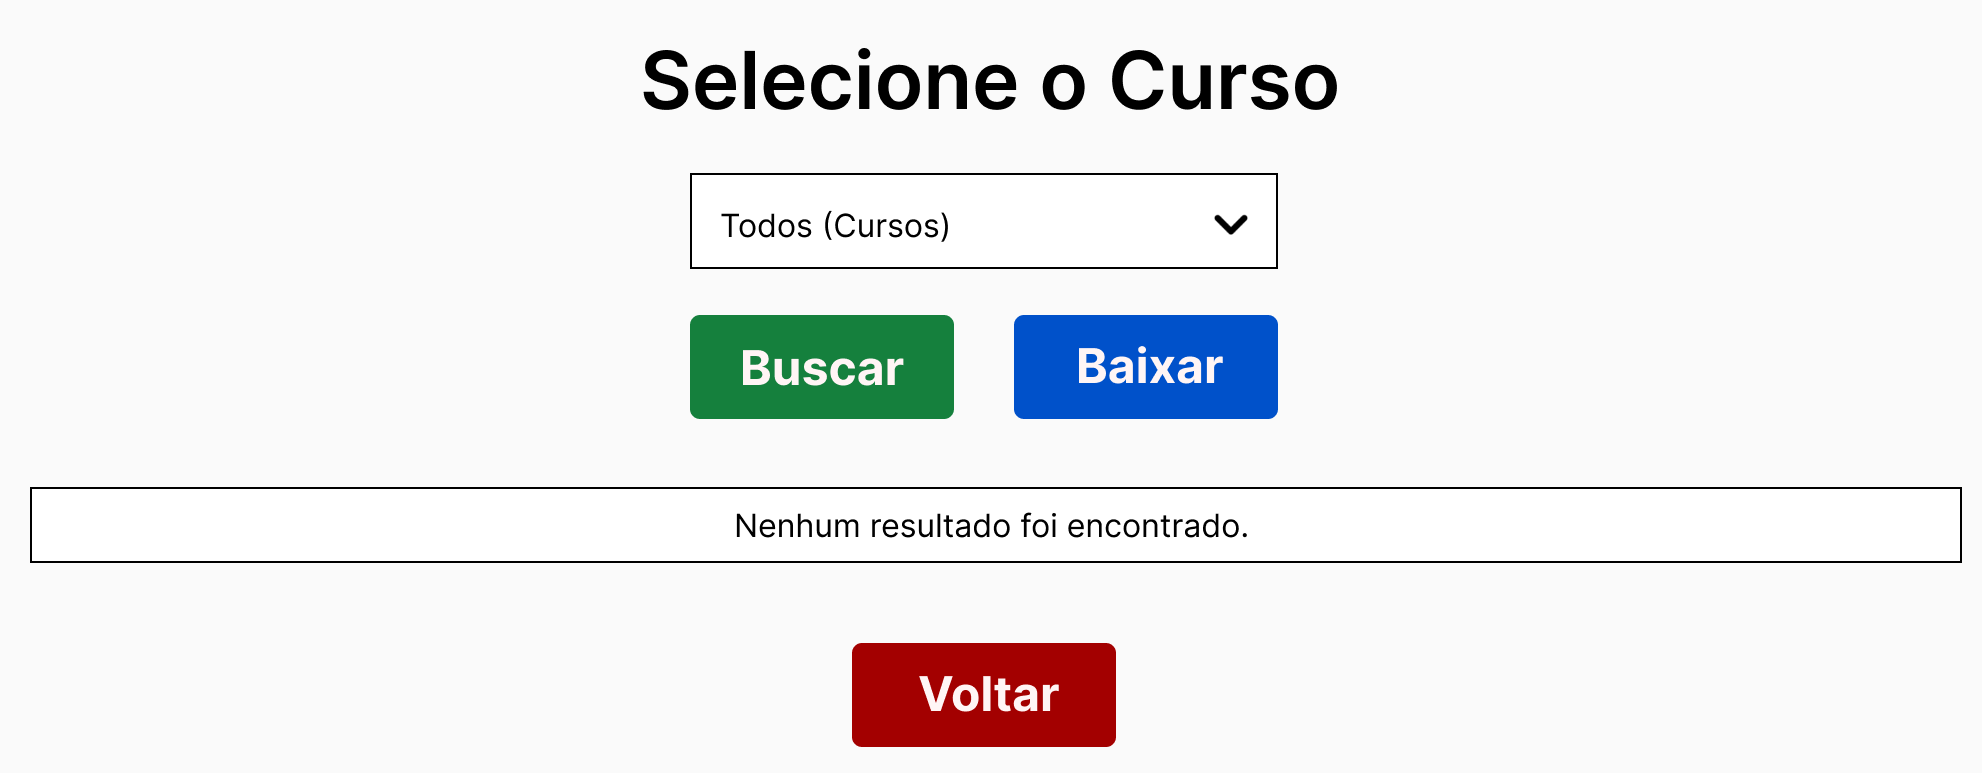
\includegraphics[width=1\textwidth]{Figuras/proto-2.PNG}
    \caption*{Fonte: Elaborado pelo autor (2024)}
    \label{fig_proto_2}
\end{figure}

\begin{figure}[htb]
    \centering
    \caption{Protótipo da tela dos cursos preenchida}
    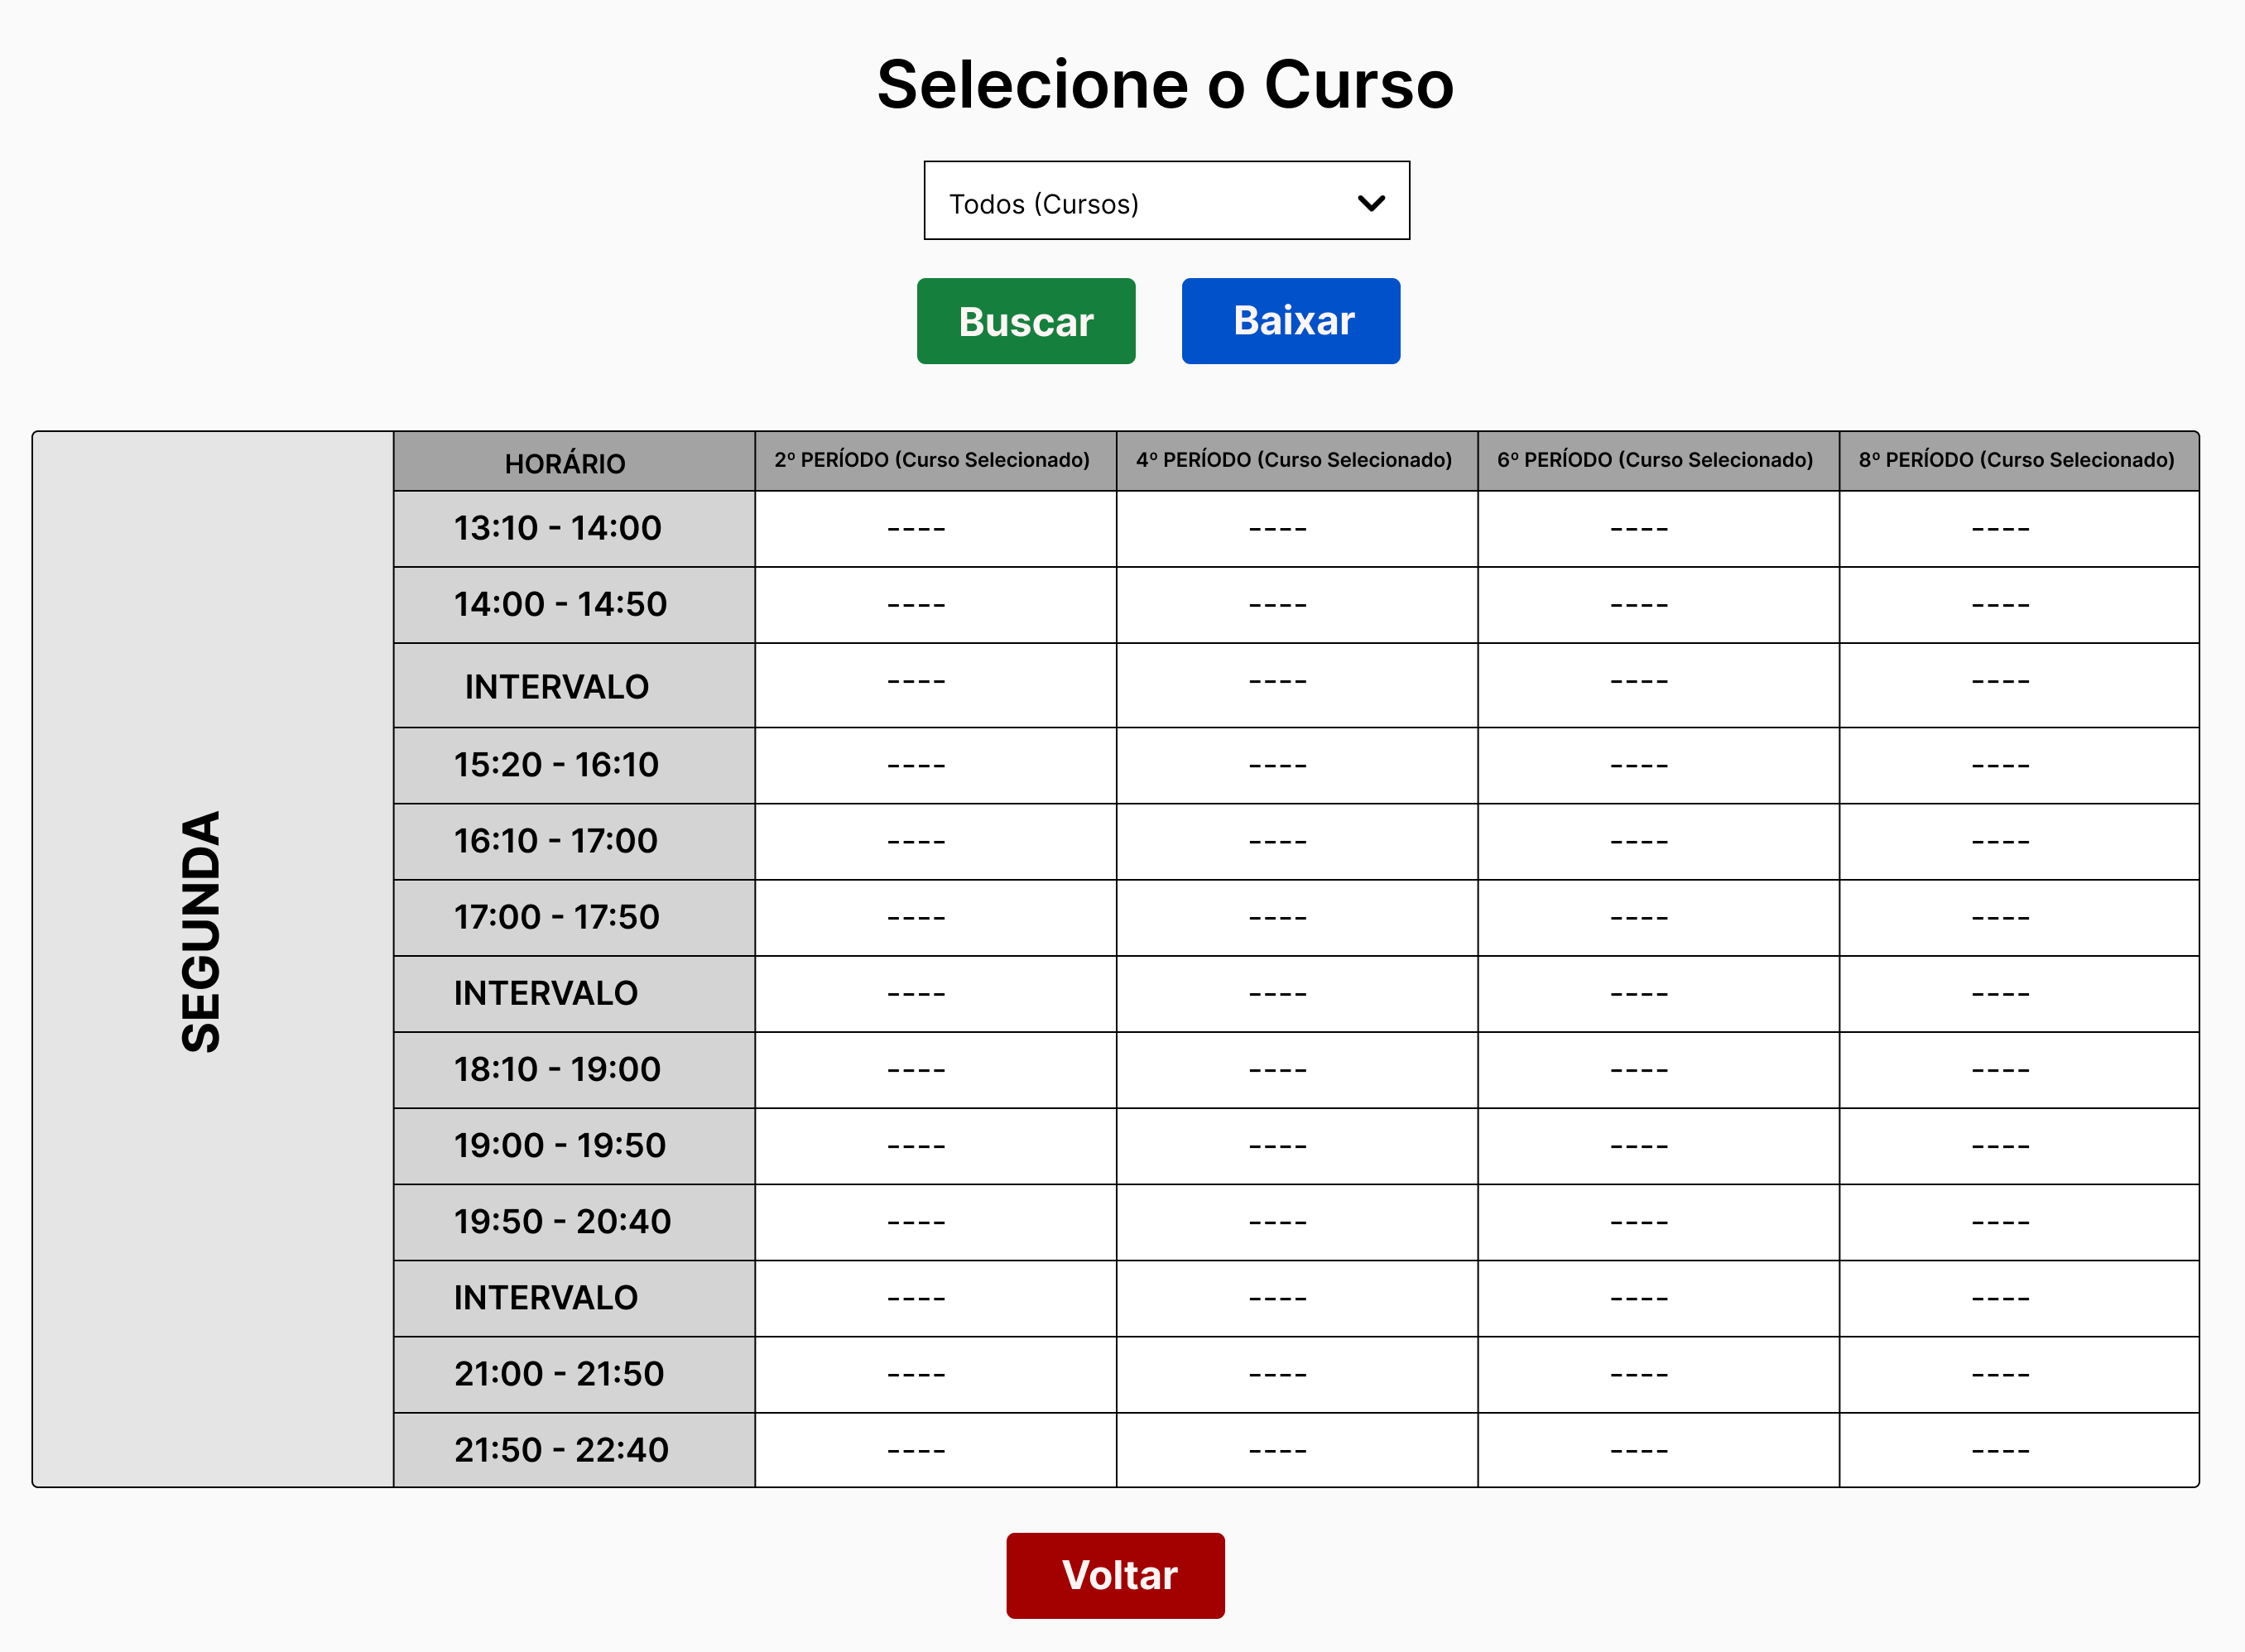
\includegraphics[width=1\textwidth]{Figuras/proto-3.PNG}
    \caption*{Fonte: Elaborado pelo autor (2024)}
    \label{fig_proto_3}
\end{figure}

As Figuras \ref{fig_proto_2} e \ref{fig_proto_3} apresentam o protótipo da tela dos cursos, exibindo os horários e a distribuição das aulas ao longo da semana para um curso selecionado.

\begin{figure}[htb]
    \centering
    \caption{Protótipo da tela dos professores}
    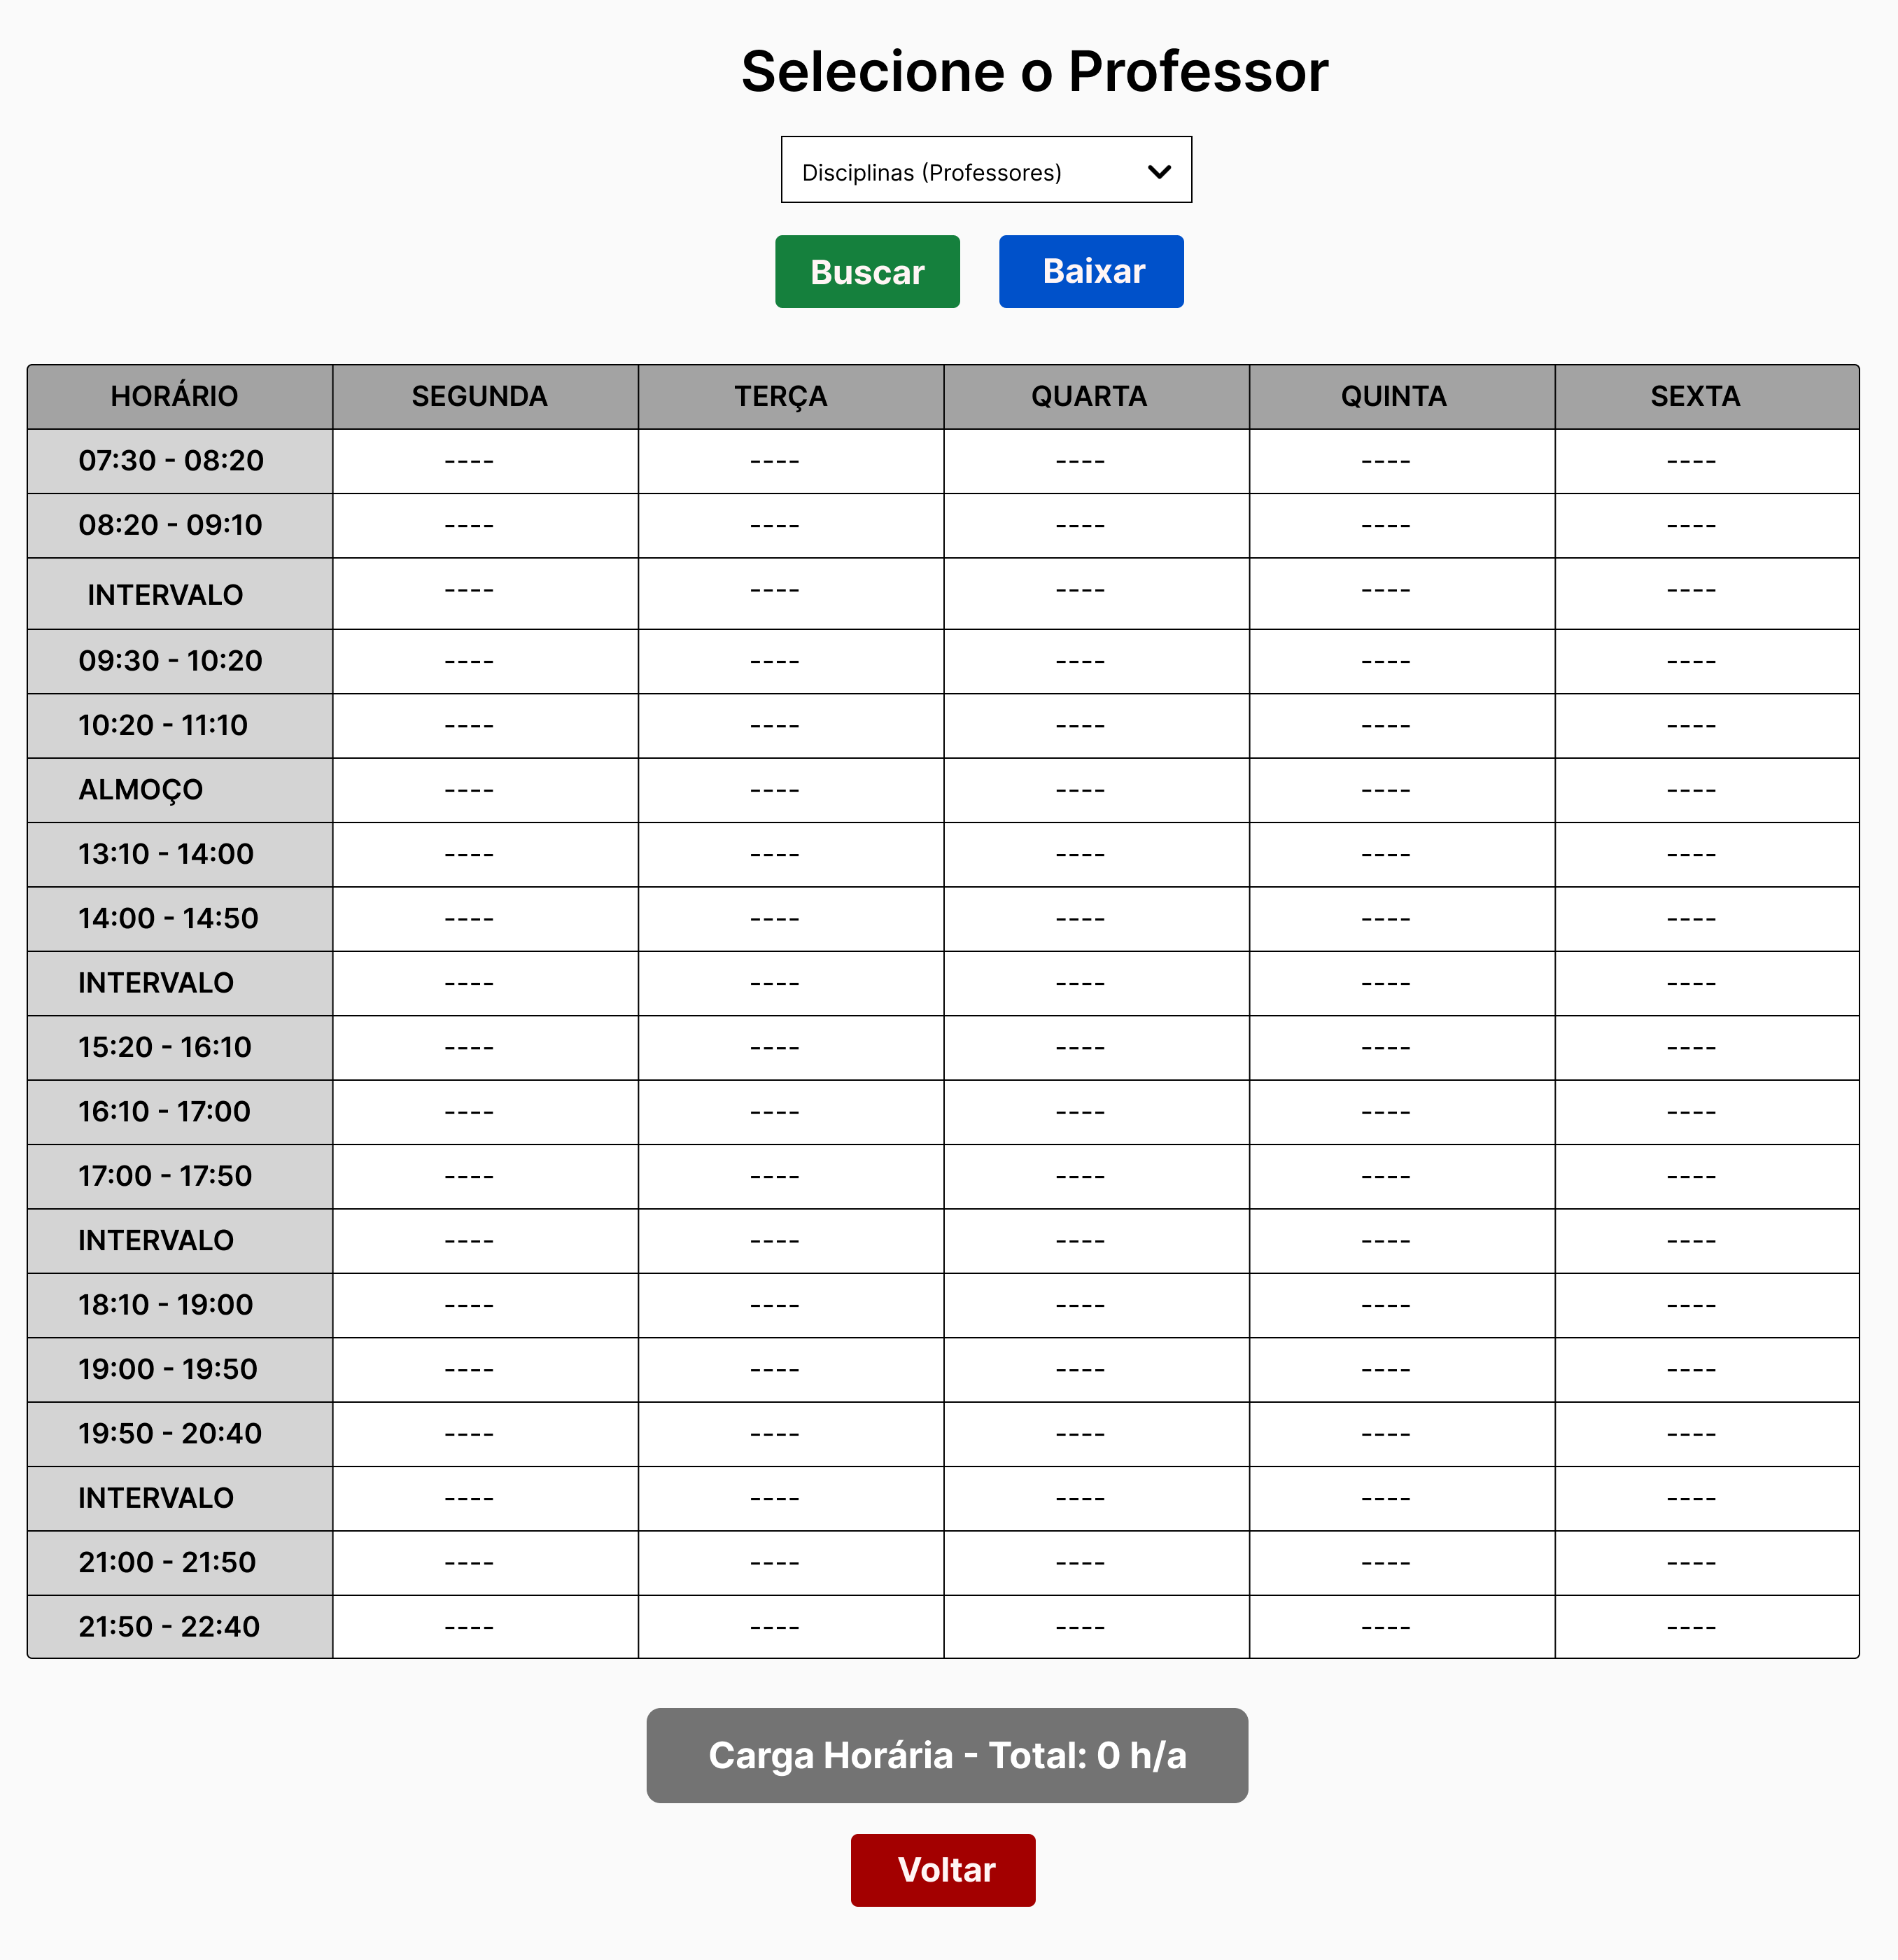
\includegraphics[width=1\textwidth]{Figuras/proto-4.PNG}
    \caption*{Fonte: Elaborado pelo autor (2024)}
    \label{fig_proto_4}
\end{figure}

A Figura \ref{fig_proto_4} apresenta o protótipo da tela dos professores, exibindo os horários das aulas e os dias da semana de um professor escolhido.

\begin{figure}[H]
    \centering
    \caption{Protótipo da tela das salas}
    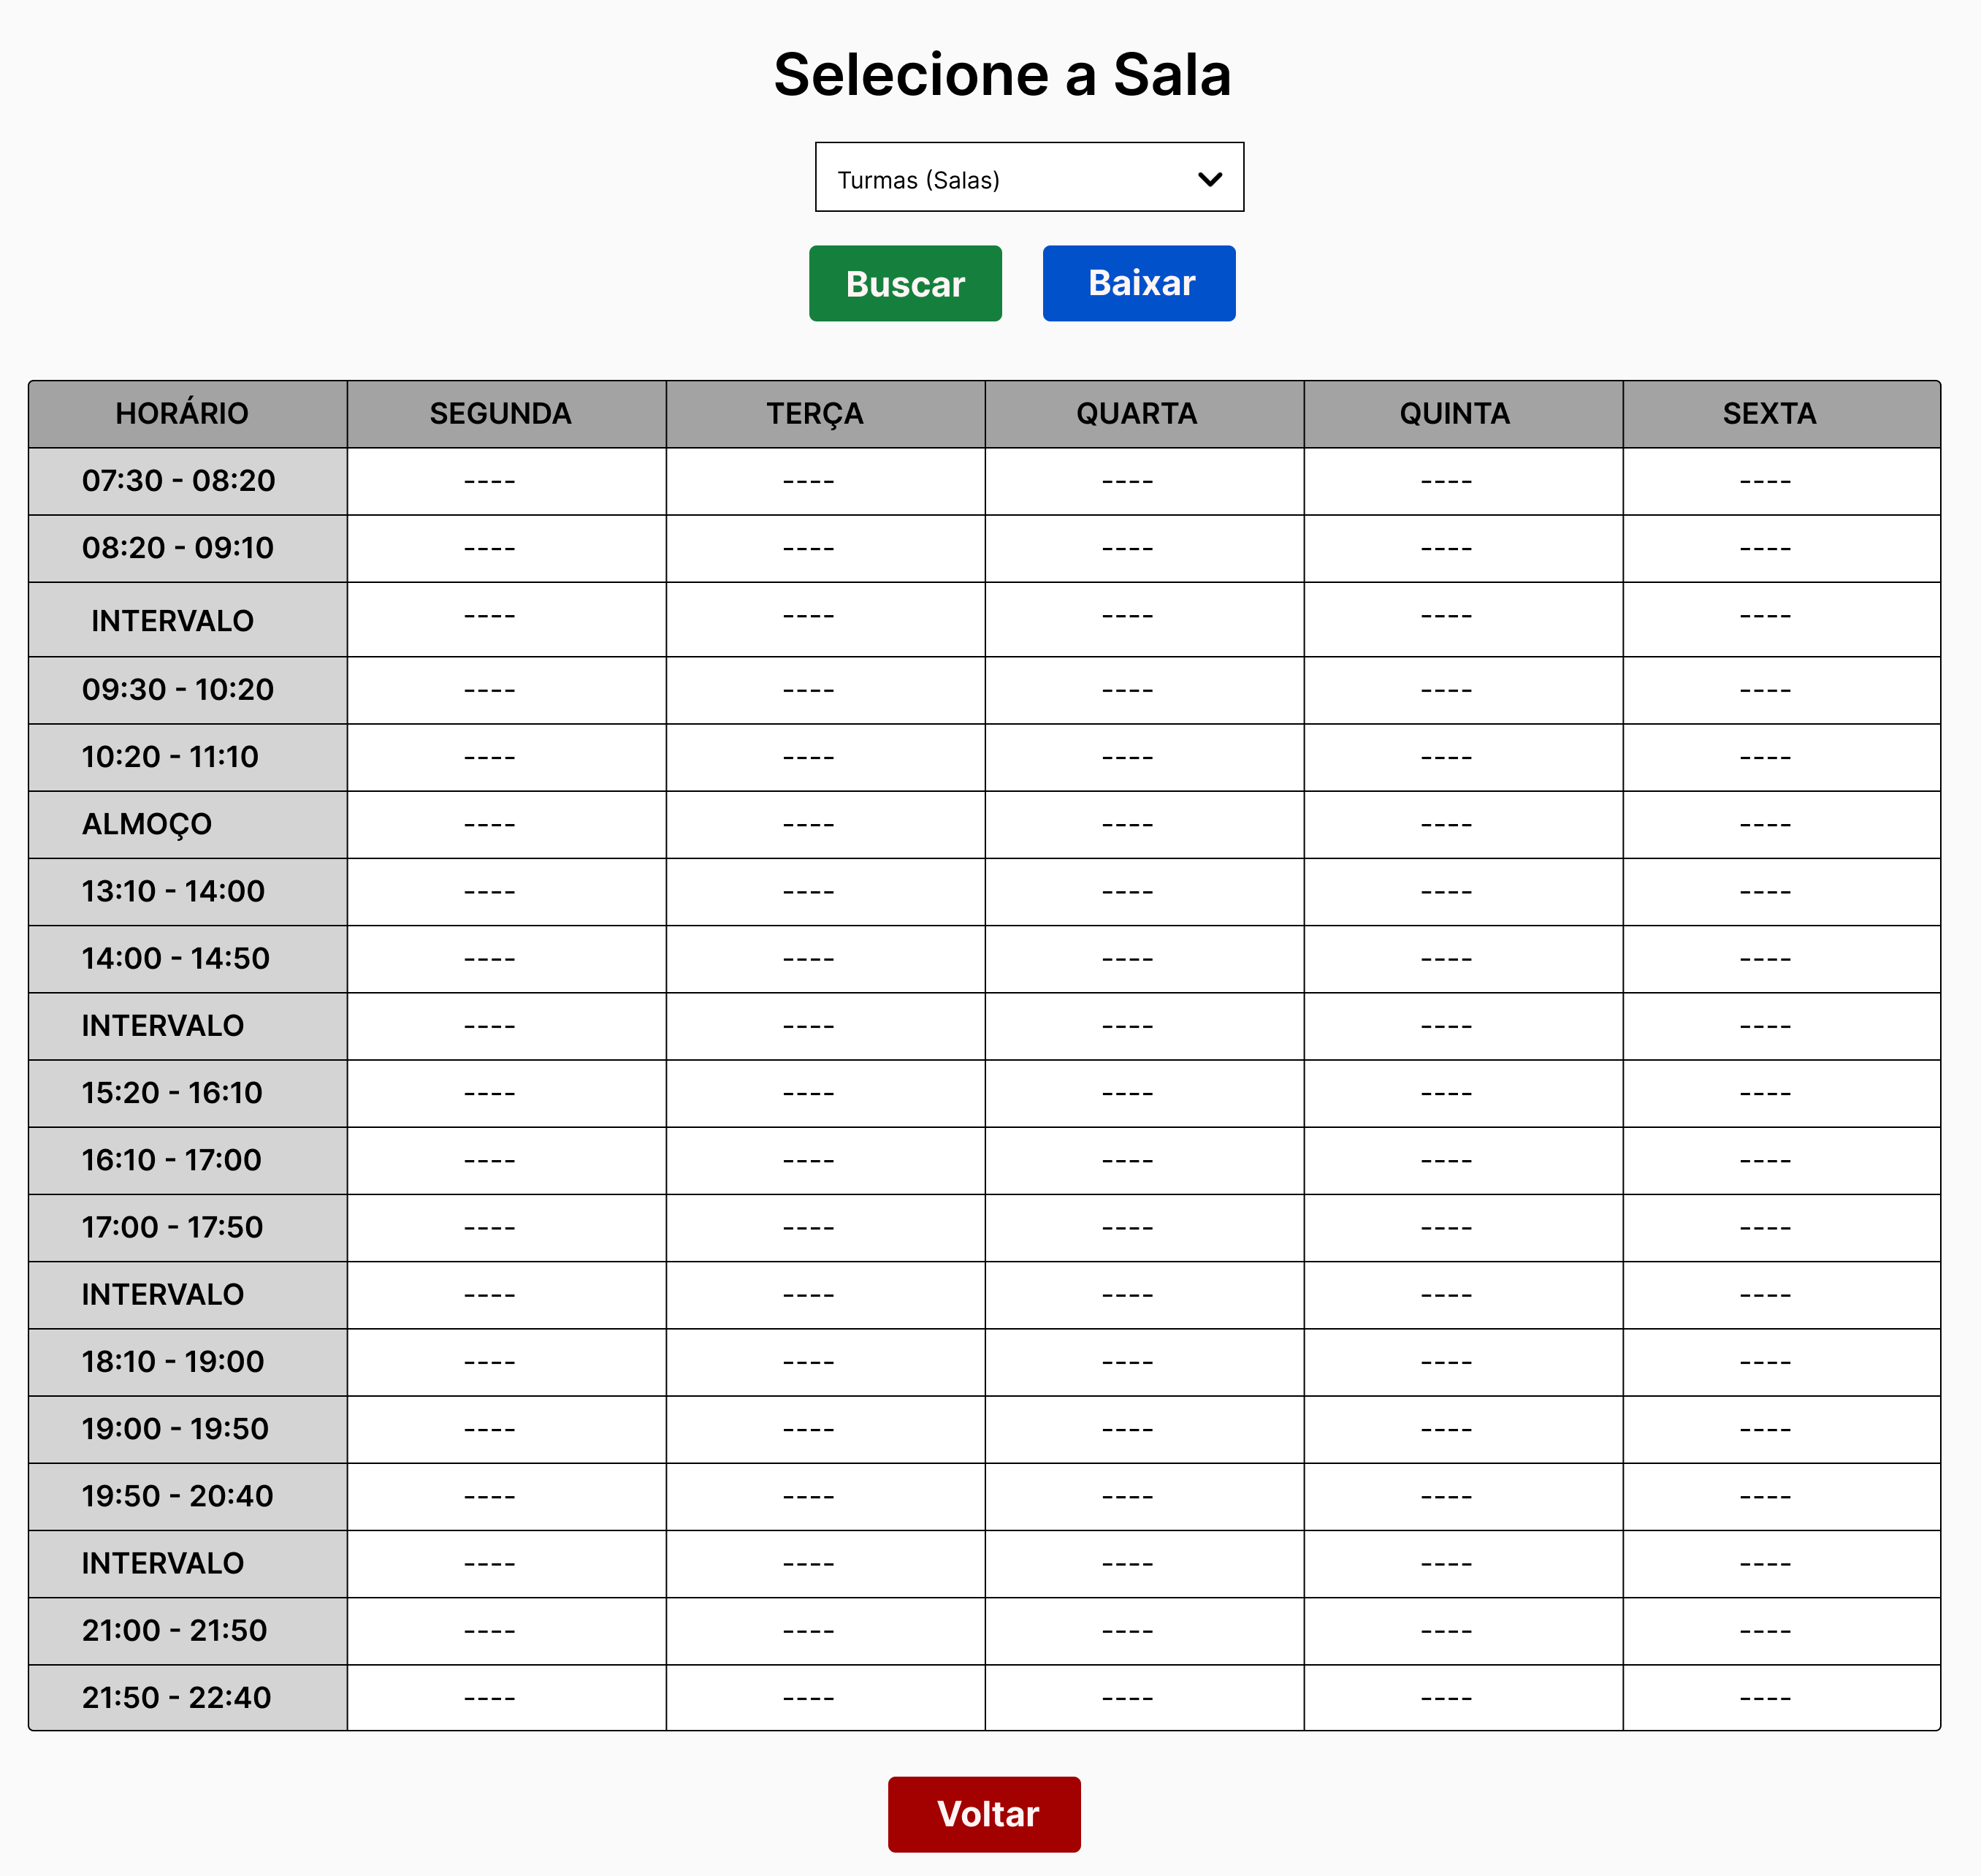
\includegraphics[width=1\textwidth]{Figuras/proto-5.PNG}
    \caption*{Fonte: Elaborado pelo autor (2024)}
    \label{fig_proto_5}
\end{figure}

A Figura \ref{fig_proto_5} apresenta o protótipo da tela das salas, exibindo os horários de ocupação e os dias em que uma sala está reservada.

\subsection{Desenvolvimento do Front-end}

O \textit{front-end} foi desenvolvido com o \textit{Next.js}. Essa tecnologia possibilitou criar uma interface moderna e eficiente, capaz de responder dinamicamente a eventos e mudanças de estado, garantindo uma experiência de usuário fluida e responsiva. Todo o trabalho priorizou clareza na organização dos componentes, reutilização de elementos e facilidade de futuras evoluções, atendendo às necessidades do projeto com agilidade. O código está disponível no repositório do projeto em: \url{https://github.com/ifnmgsal-inf/Horarios-IFNMG-Salinas/tree/main/frontend}. A seguir, são exibidas as telas resultantes desse processo:

\begin{figure}[htb]
    \centering
    \caption{Menu principal com opções de botões de horários e outros serviços}
    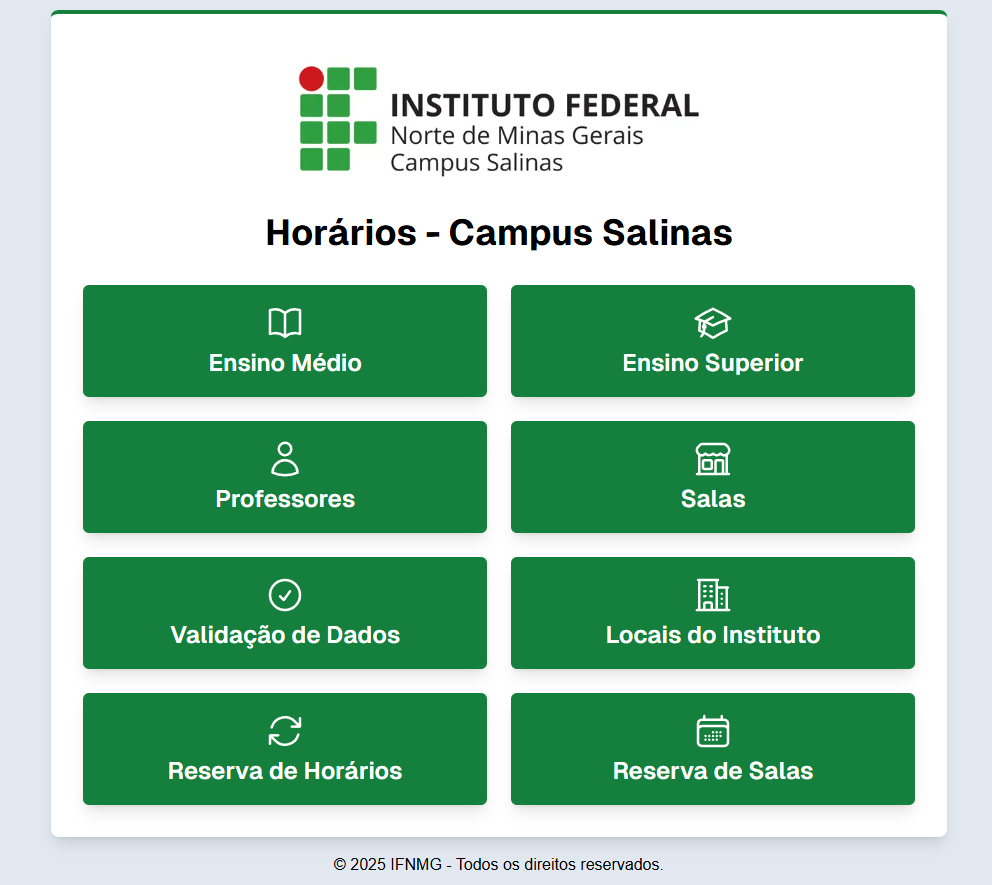
\includegraphics[width=1\textwidth]{Figuras/front-1.png}
    \caption*{Fonte: Elaborado pelo autor (2025)}
    \label{fig_front_1}
\end{figure}

A Figura \ref{fig_front_1} mostra o menu principal da plataforma, com botões para consulta de horários e acesso a outros serviços.

\begin{figure}[htb]
    \centering
    \caption{Tela dos cursos}
    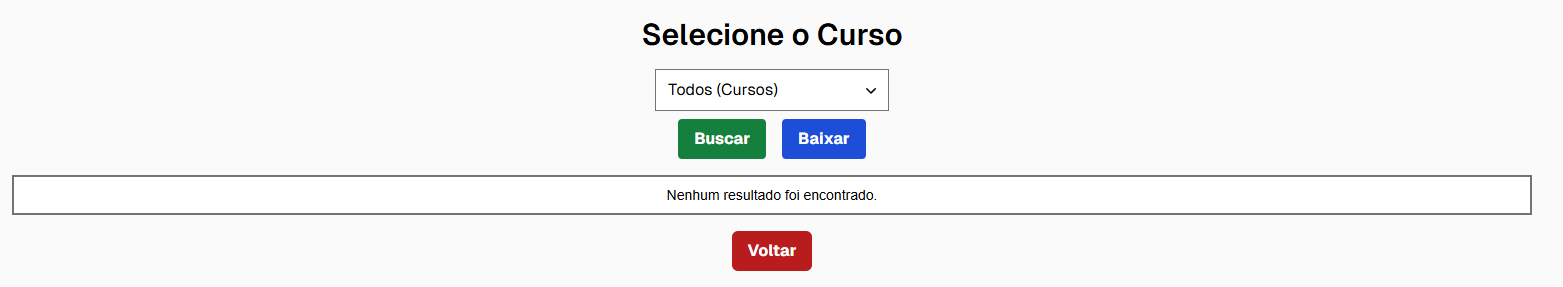
\includegraphics[width=1\textwidth]{Figuras/front-2.png}
    \caption*{Fonte: Elaborado pelo autor (2025)}
    \label{fig_front_2}
\end{figure}

A Figura \ref{fig_front_2} mostra a tela dos cursos com nenhum curso selecionado.

\begin{figure}[htb]
    \centering
    \caption{Tela dos cursos com cursos técnicos}
    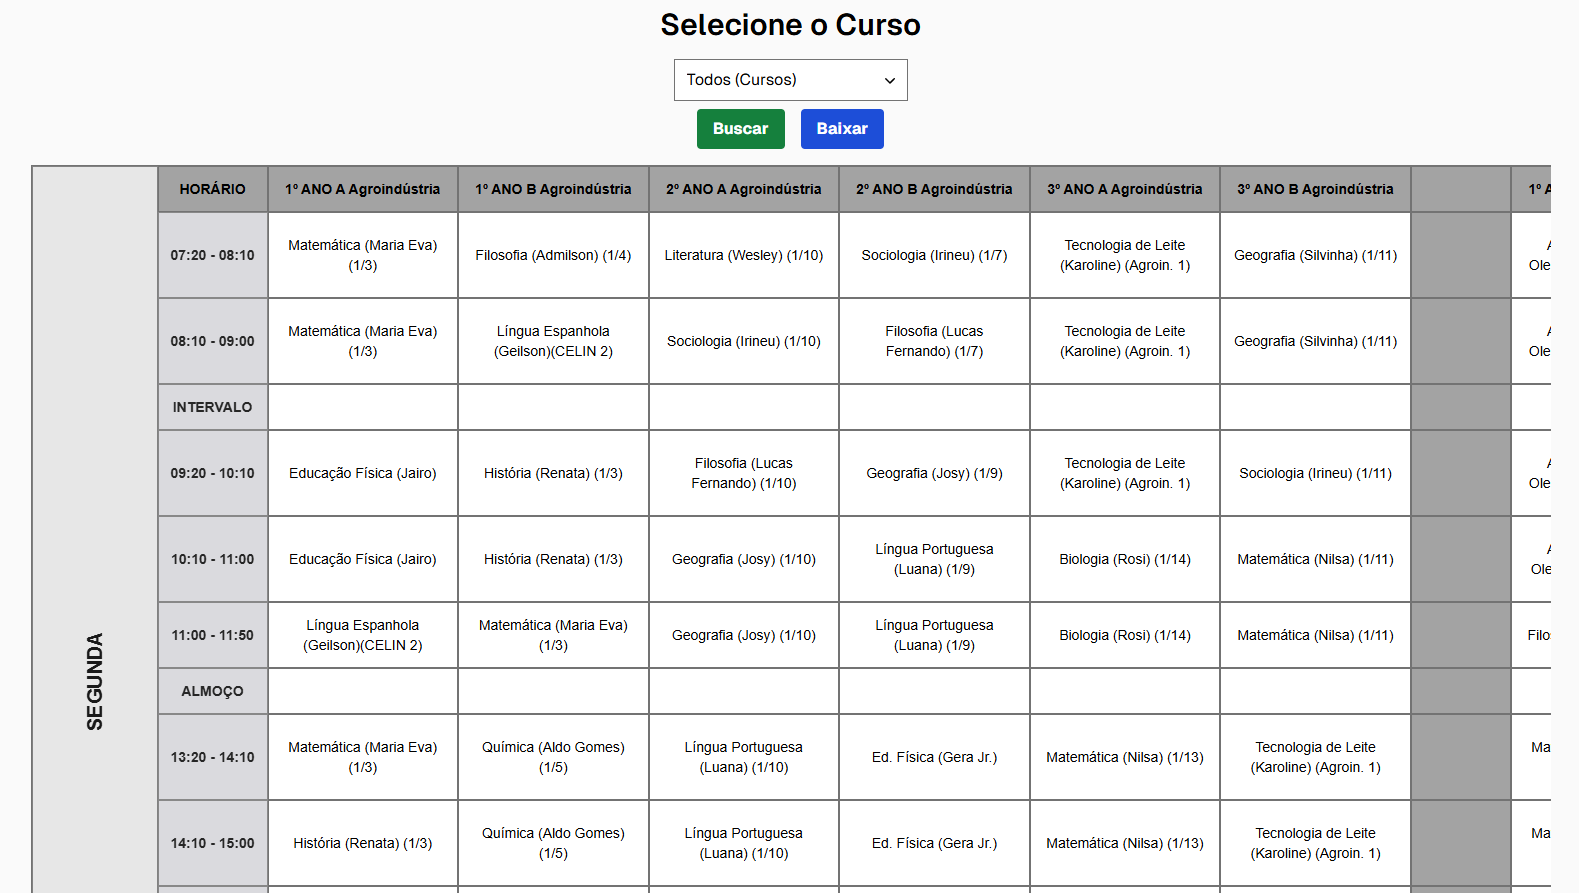
\includegraphics[width=1\textwidth]{Figuras/front-3.png}
    \caption*{Fonte: Elaborado pelo autor (2025)}
    \label{fig_front_3}
\end{figure}

\begin{figure}[H]
    \centering
    \caption{Tela dos cursos com cursos superiores}
    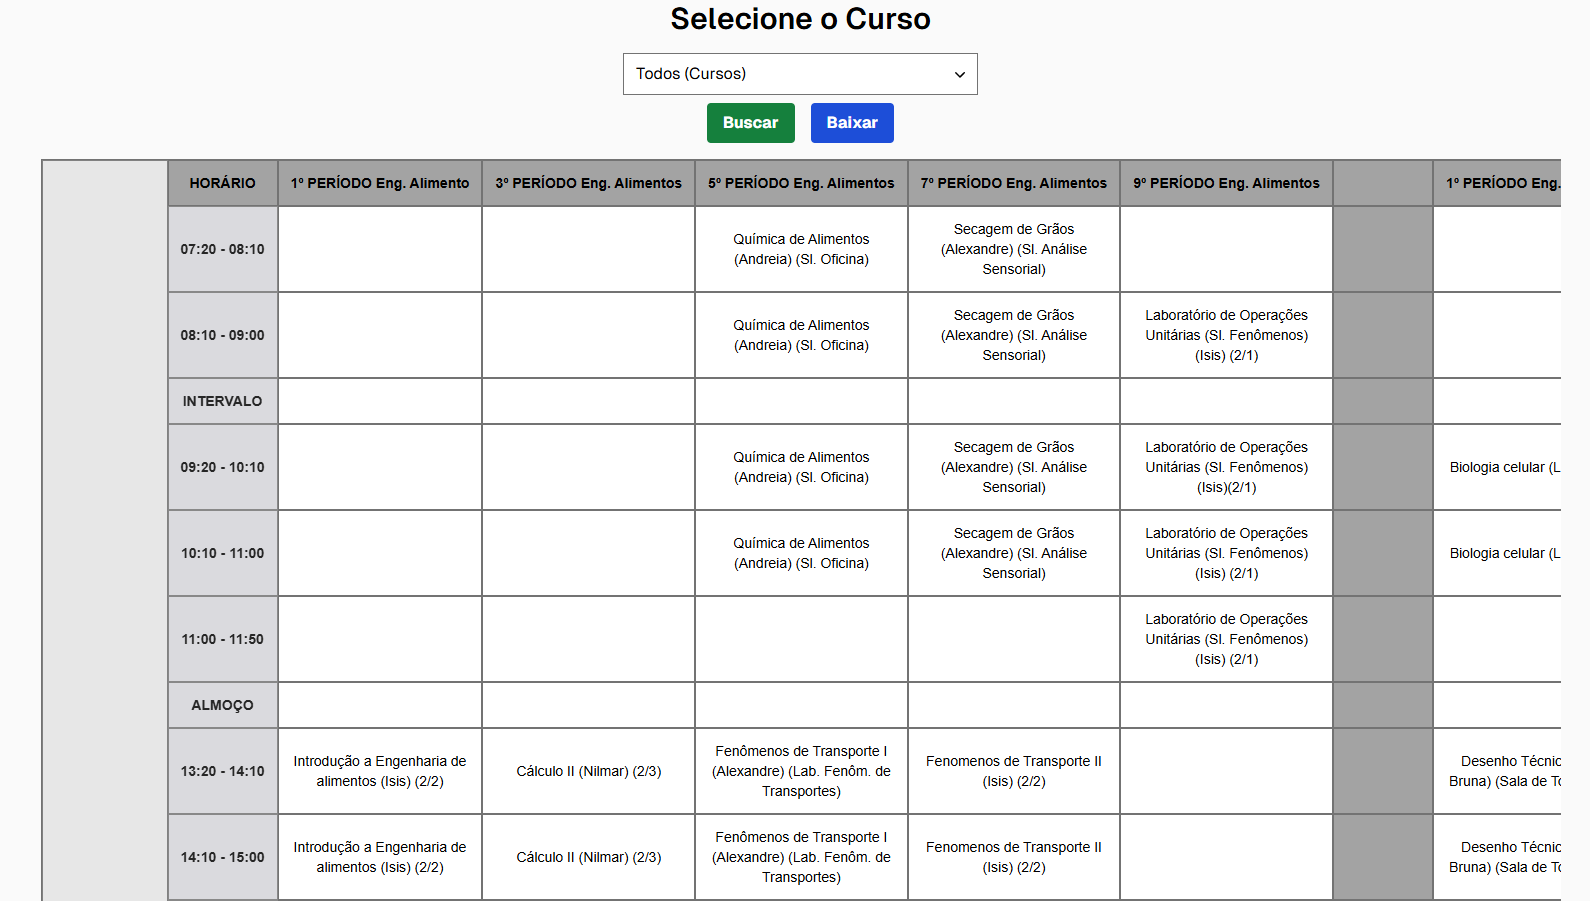
\includegraphics[width=1\textwidth]{Figuras/front-4.png}
    \caption*{Fonte: Elaborado pelo autor (2025)}
    \label{fig_front_4}
\end{figure}

As Figuras \ref{fig_front_3} e \ref{fig_front_4} mostram a tela dos cursos com os horários dos cursos técnicos e superiores com as turmas e os dias da semana.

\begin{figure}[htb]
    \centering
    \caption{Tela dos professores}
    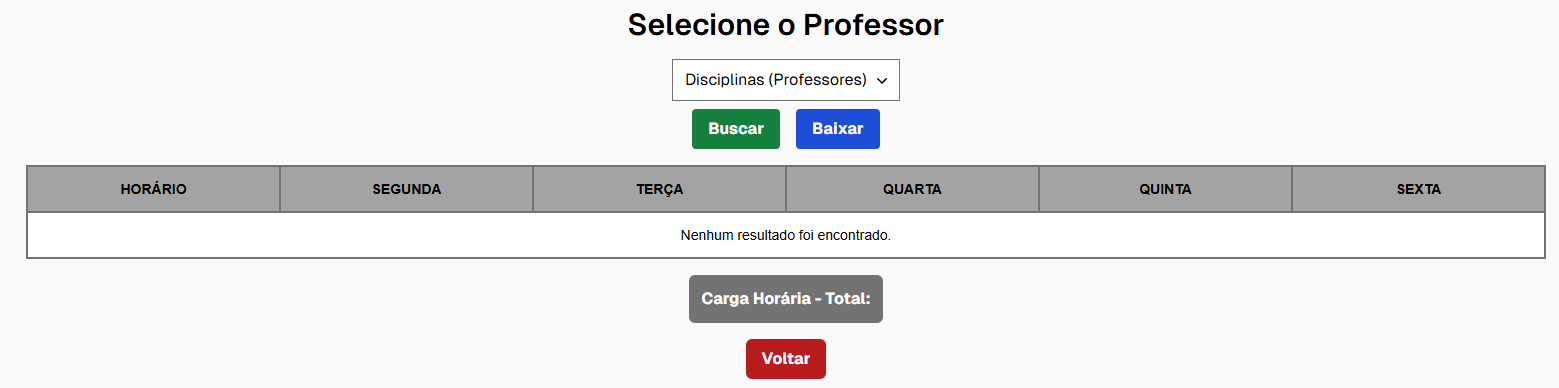
\includegraphics[width=1\textwidth]{Figuras/front-5.png}
    \caption*{Fonte: Elaborado pelo autor (2025)}
    \label{fig_front_5}
\end{figure}

\begin{figure}[H]
    \centering
    \caption{Tela dos professores com um professor selecionado}
    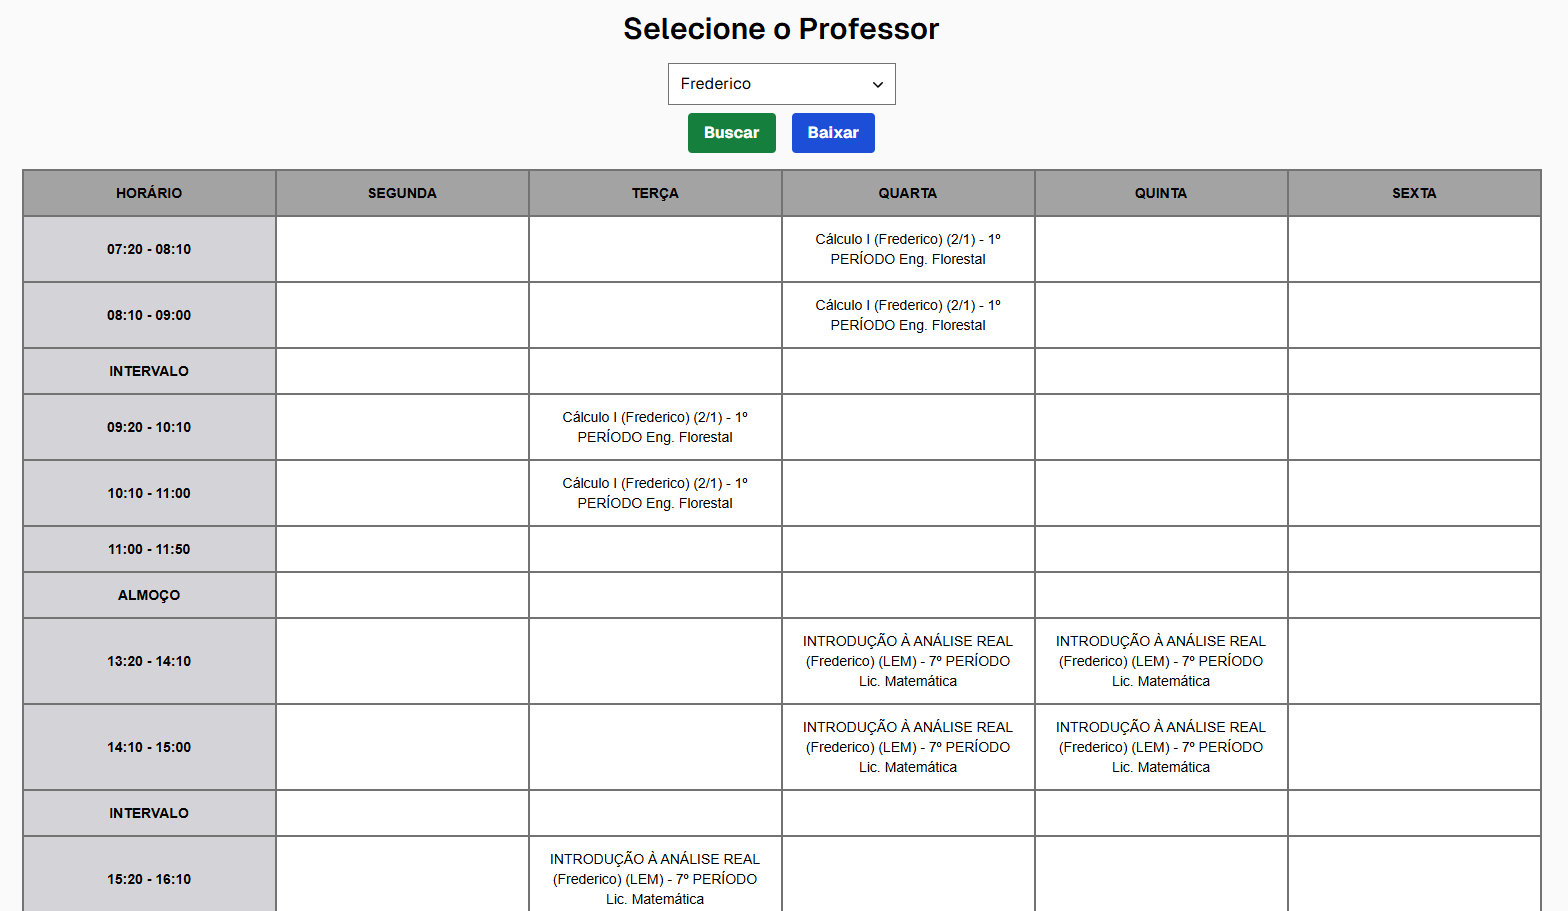
\includegraphics[width=1\textwidth]{Figuras/front-6.png}
    \caption*{Fonte: Elaborado pelo autor (2025)}
    \label{fig_front_6}
\end{figure}

A Figura \ref{fig_front_5} mostra a tela dos professores com nenhum professor selecionado e a Figura \ref{fig_front_6} exibe um professor selecionado, com seus horários semanais.

\begin{figure}[H]
    \centering
    \caption{Tela das salas}
    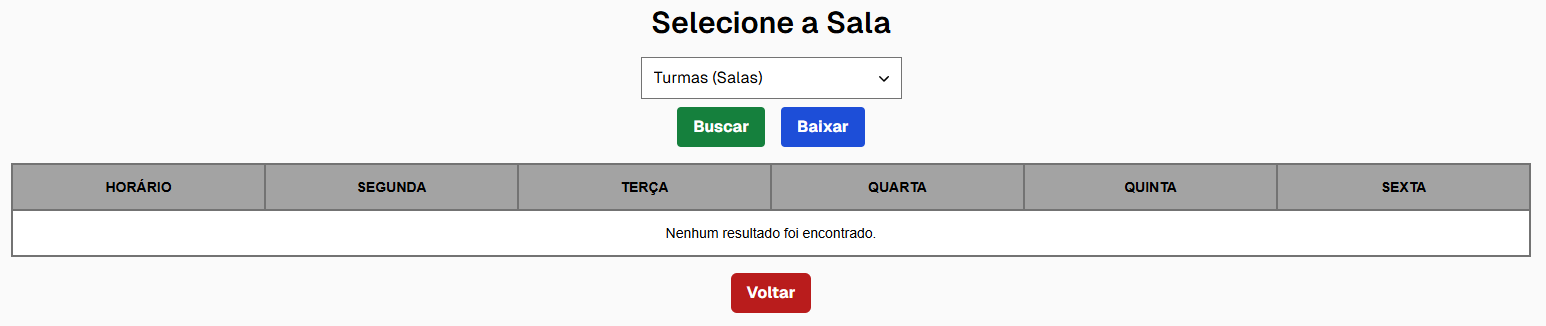
\includegraphics[width=1\textwidth]{Figuras/front-7.png}
    \caption*{Fonte: Elaborado pelo autor (2025)}
    \label{fig_front_7}
\end{figure}

\begin{figure}[htb]
    \centering
    \caption{Tela das salas com uma sala selecionada}
    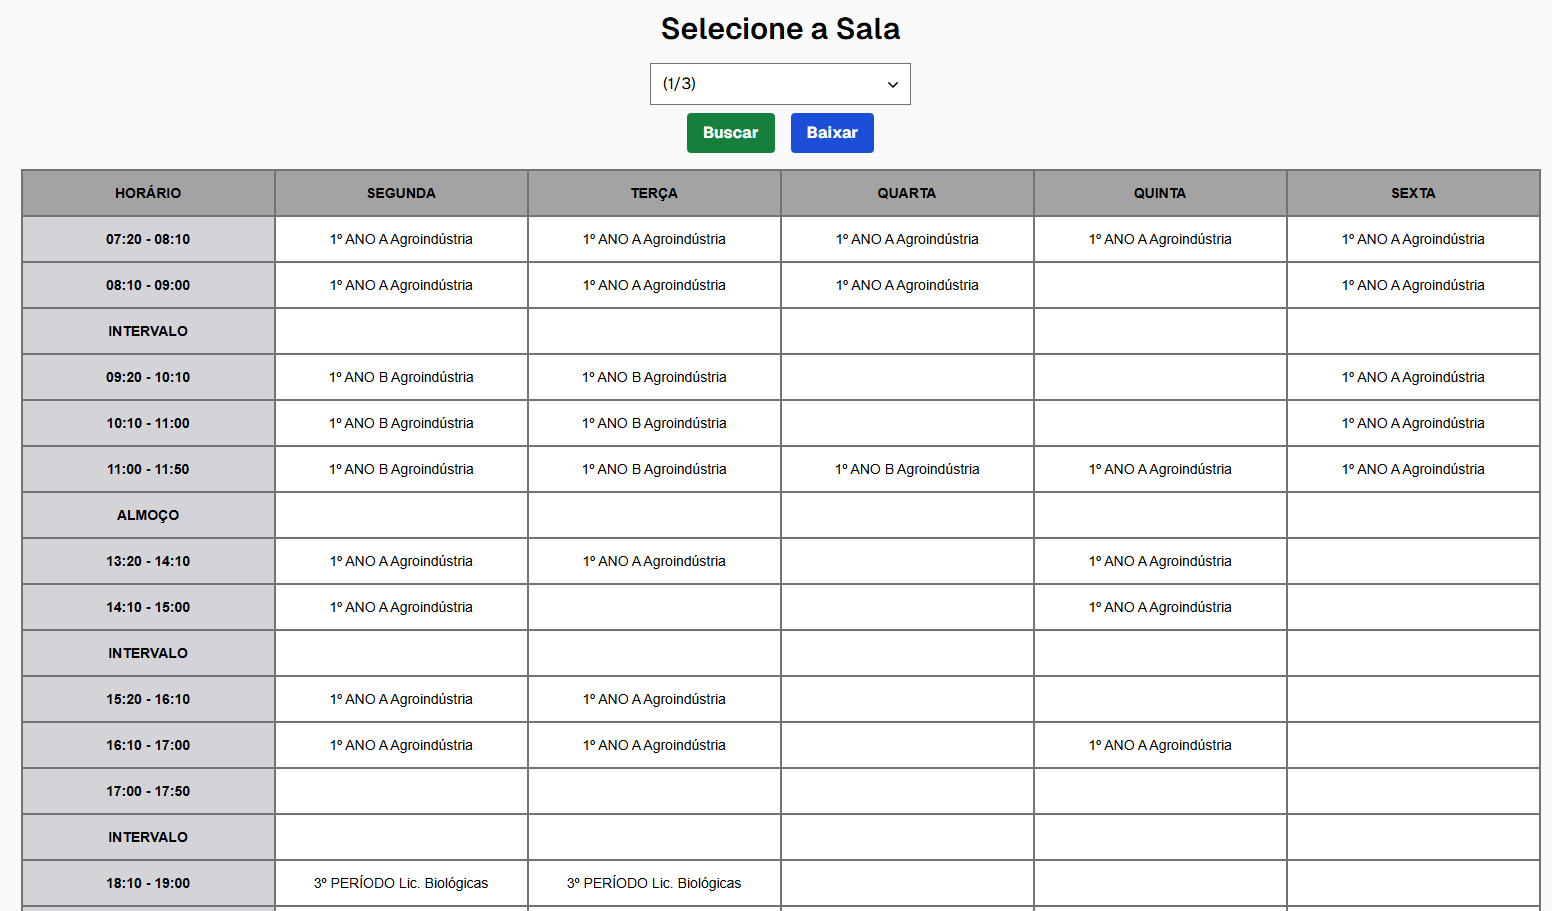
\includegraphics[width=1\textwidth]{Figuras/front-8.png}
    \caption*{Fonte: Elaborado pelo autor (2025)}
    \label{fig_front_8}
\end{figure}

A Figura \ref{fig_front_7} mostra a tela das salas com nenhuma sala selecionada e a Figura \ref{fig_front_8} exibe uma sala selecionada com seus horários de ocupação semanais.

\begin{figure}[htb]
    \centering
    \caption{Tela de login}
    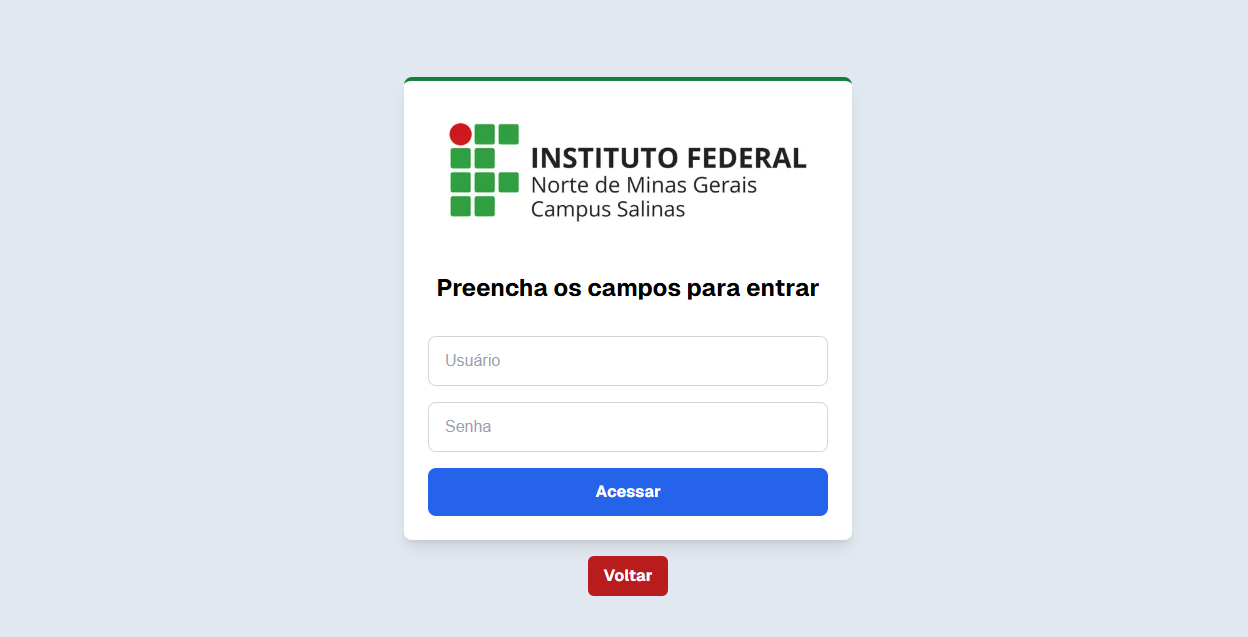
\includegraphics[width=1\textwidth]{Figuras/front-9.png}
    \caption*{Fonte: Elaborado pelo autor (2025)}
    \label{fig_front_9}
\end{figure}

\begin{figure}[H]
    \centering
    \caption{Tela de validação de dados}
    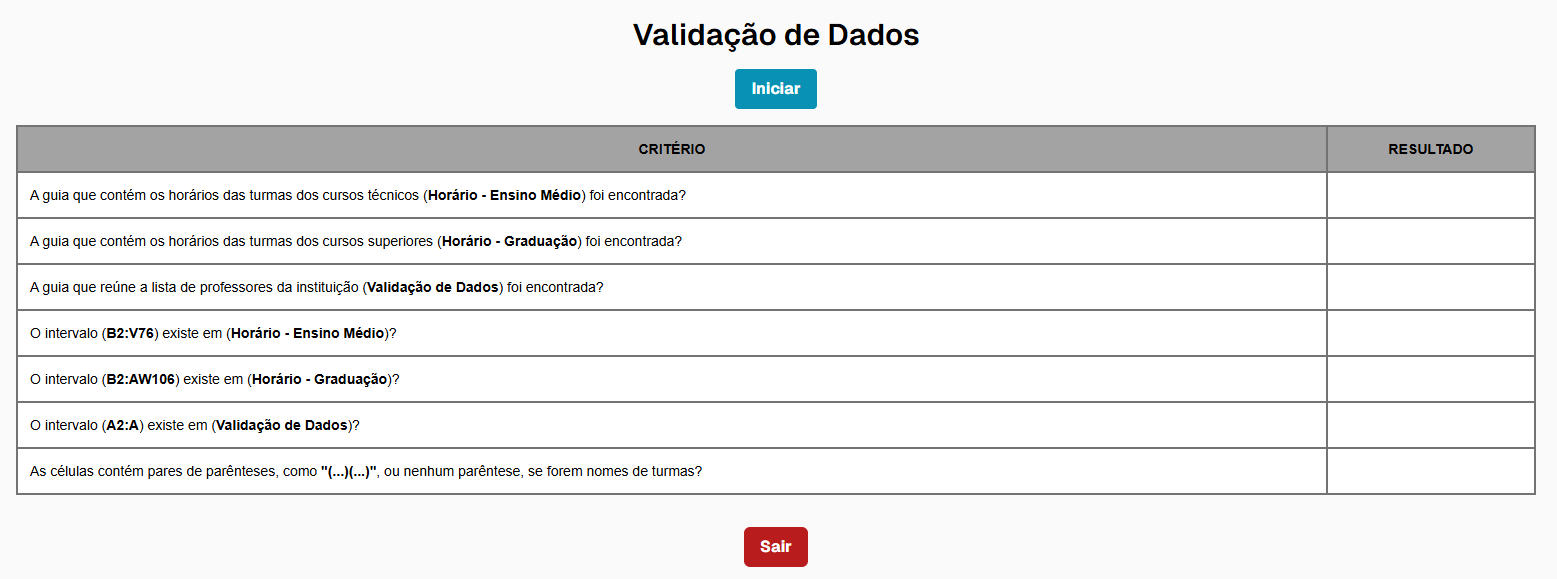
\includegraphics[width=1\textwidth]{Figuras/front-10.png}
    \caption*{Fonte: Elaborado pelo autor (2025)}
    \label{fig_front_10}
\end{figure}

Já a Figura \ref{fig_front_9} mostra a tela de login para acessar a tela de validação de dados, e a Figura \ref{fig_front_10} exibe a tela de validação de dados com critérios e os resultados que podem ser obtidos a partir da planilha.

\begin{figure}[htb]
    \centering
    \caption{Sistema que exibe os locais do instituto}
    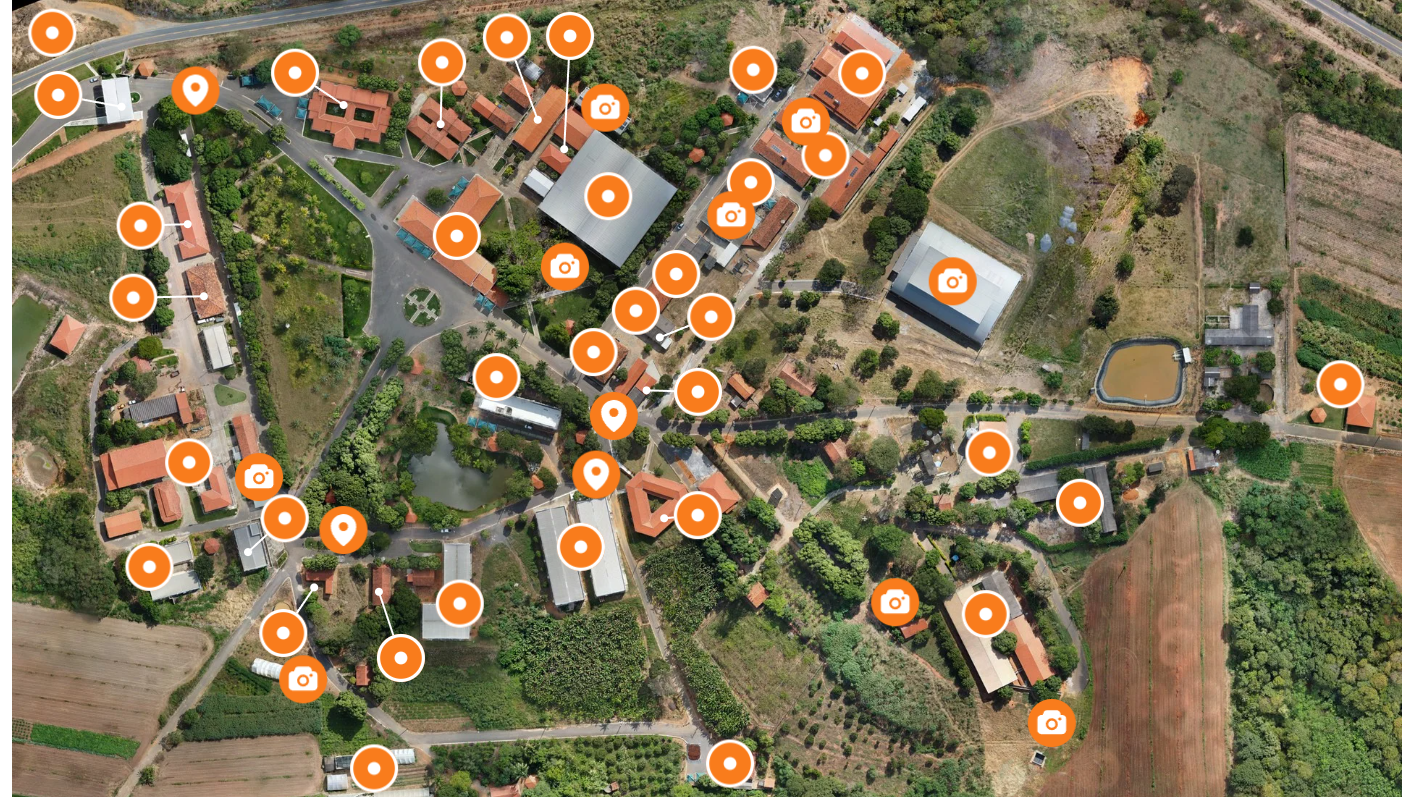
\includegraphics[width=1\textwidth]{Figuras/front-11.png}
    \caption*{Fonte: Elaborado pelo autor (2025)}
    \label{fig_front_11}
\end{figure}

\begin{figure}[H]
    \centering
    \caption{Sistema de reserva de horários}
    
\includegraphics[width=1\textwidth]{Figuras/front-12.png}
    \caption*{Fonte: Elaborado pelo autor (2025)}
    \label{fig_front_12}
\end{figure}

\begin{figure}[htb]
    \centering
    \caption{Sistema de gerenciamento de reserva de salas}
    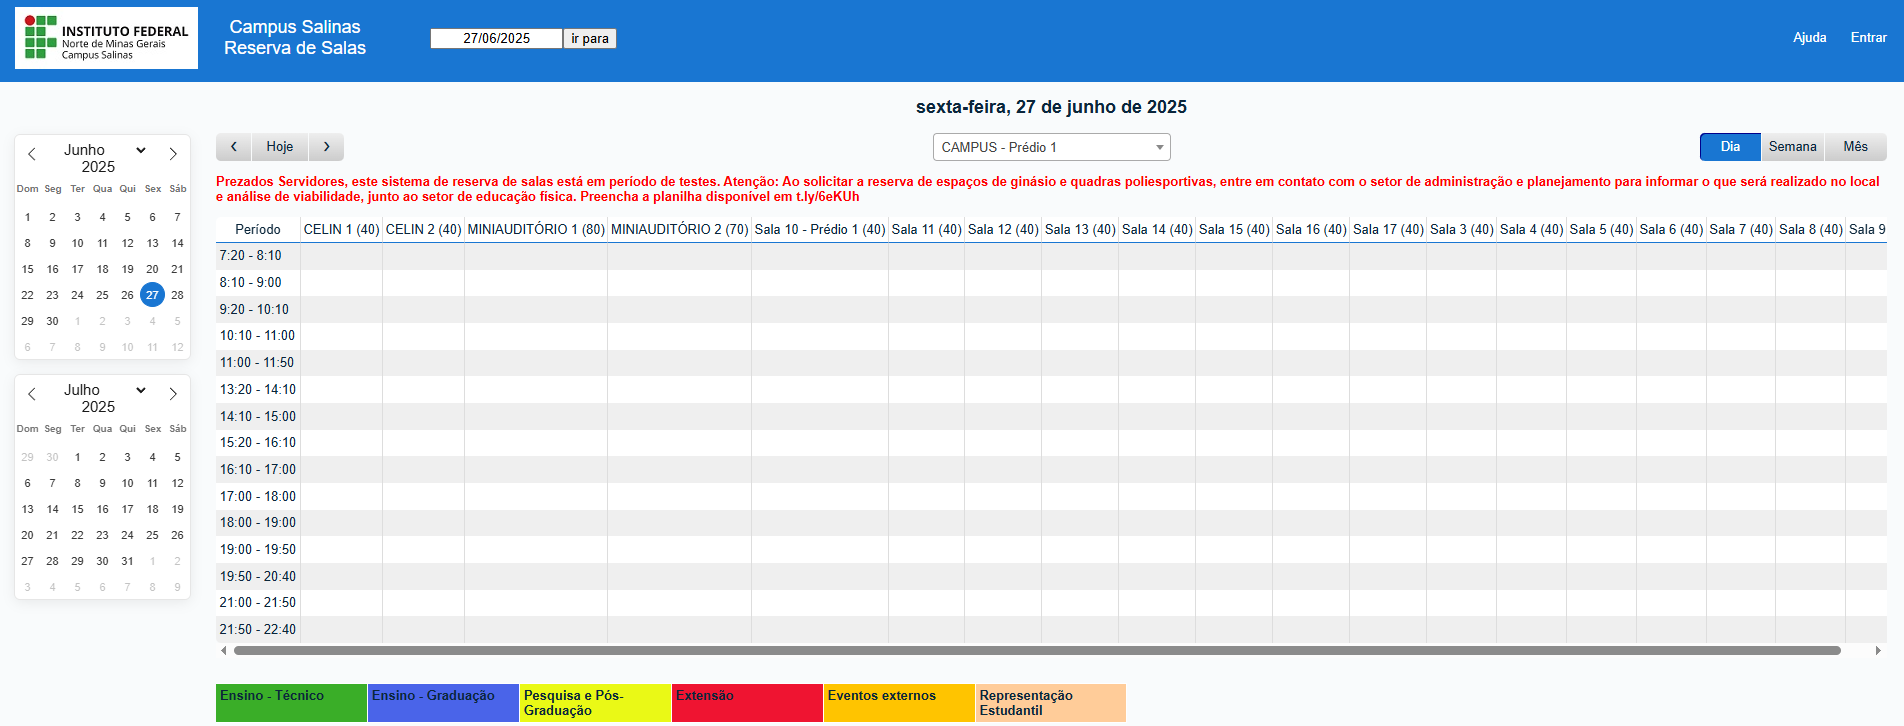
\includegraphics[width=1\textwidth]{Figuras/front-13.png}
    \caption*{Fonte: Elaborado pelo autor (2025)}
    \label{fig_front_13}
\end{figure}

Por fim, as Figuras \ref{fig_front_11}, \ref{fig_front_12} e \ref{fig_front_13} apresentam os sistemas externos integrados à plataforma, incluindo a visualização de locais do instituto, o sistema de reserva de horários e o gerenciamento de reservas de salas. Esses sistemas, embora estejam acessíveis a partir da plataforma desenvolvida, não estão incluídos no escopo desse trabalho.

\subsection{Estrutura do Front-end}

A estrutura do \textit{front-end} está organizada de forma modular, visando clareza, manutenção facilitada e reutilização de código. Na Figura \ref{fig_front_14}, destacam-se os principais elementos:

\begin{figure}[htb]
    \centering
    \caption{Estrutura do front-end}
    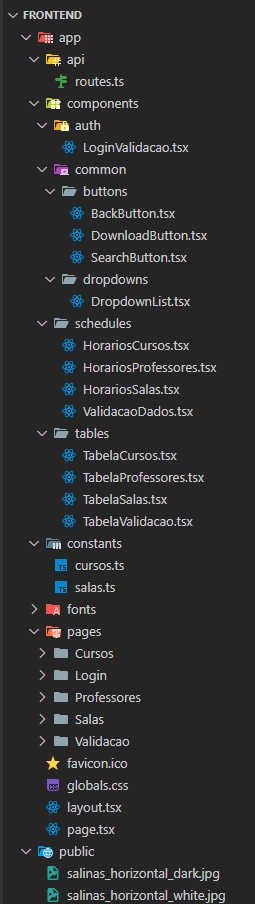
\includegraphics[width=0.3\textwidth]{Figuras/front-14.png}
    \caption*{Fonte: Elaborado pelo autor (2025)}
    \label{fig_front_14}
\end{figure}

\begin{itemize}
    \item \textbf{api}: pasta responsável por buscar dados da planilha por meio de requisições, contando com o arquivo \textit{routes.ts}, que gerencia essas chamadas e contém a variável de ambiente para comunicação com o \textit{back-end}.
    \item components: pasta que centraliza os componentes do sistema, subdividida em:
    \begin{itemize}
        \item \textbf{auth}: pasta responsável pelo controle de autenticação, incluindo o componente \textit{LoginValidacao.tsx}, que verifica as credenciais de login antes de entrar na tela de validação.
        \item \textbf{common}: pasta destinada a componentes reutilizáveis, contendo:
        \begin{itemize}
            \item \textbf{buttons}: reúne botões de ação como \textit{BackButton.tsx} para retorno, \textit{DownloadButton.tsx} para download de tabelas e \textit{SearchButton.tsx} para busca de horários.
             \item \textbf{dropdowns}: responsável pelas listas suspensas, como o componente \textit{DropdownList.tsx}, utilizado para seleção de cursos, professores ou salas.
        \end{itemize}
        \item \textbf{schedules}: pasta com componentes independentes para exibição de horários organizados por tipo de consulta, como \textit{HorariosCursos.tsx}, \textit{HorariosProfessores.tsx} e \textit{HorariosSalas.tsx}, que apresentam uma lista suspensa para seleção e uma tabela com os horários correspondentes, e \textit{ValidacaoDados.tsx}, que exibe a tabela com os resultados da validação da planilha dos horários.
        \item \textbf{tables}: pasta com componentes independentes das tabelas com os dados, incluindo \textit{TabelaCursos.tsx}, \textit{TabelaProfessores.tsx}, \textit{TabelaSalas.tsx} e \textit{TabelaValidacao.tsx}.
    \end{itemize}
    \item \textbf{constants}: pasta responsável por definir as listas de cursos e salas disponíveis, armazenadas nos arquivos \textit{cursos.ts} e \textit{salas.ts}.
    \item \textbf{pages}: pasta que organiza as rotas da aplicação, com páginas específicas para cursos, professores, salas, login e validação.
    \item \textbf{globals.css}: arquivo de estilos globais aplicados em toda a interface.
    \item \textbf{layout.tsx}: componente que define a estrutura geral de layout e permite a edição de metadados de forma centralizada.
    \item \textbf{page.tsx}: componente com página inicial que exibe o menu principal com opções de botões de horários e outros serviços.
    \item \textbf{public}: pasta com imagens do logotipo institucional do IFNMG Campus Salinas, disponibilizadas tanto na versão padrão quanto na versão em preto e branco.
\end{itemize}

\subsection{Funcionalidades do Front-end}

\begin{itemize}
    \item \textbf{Modo escuro}: adapta automaticamente o tema da aplicação entre claro ou escuro, de acordo com a configuração do navegador, oferecendo maior conforto visual aos usuários. Apresentado na Figura \ref{fig_front_15}.

    \begin{figure}[htb]
        \centering
        \caption{Modo escuro}
        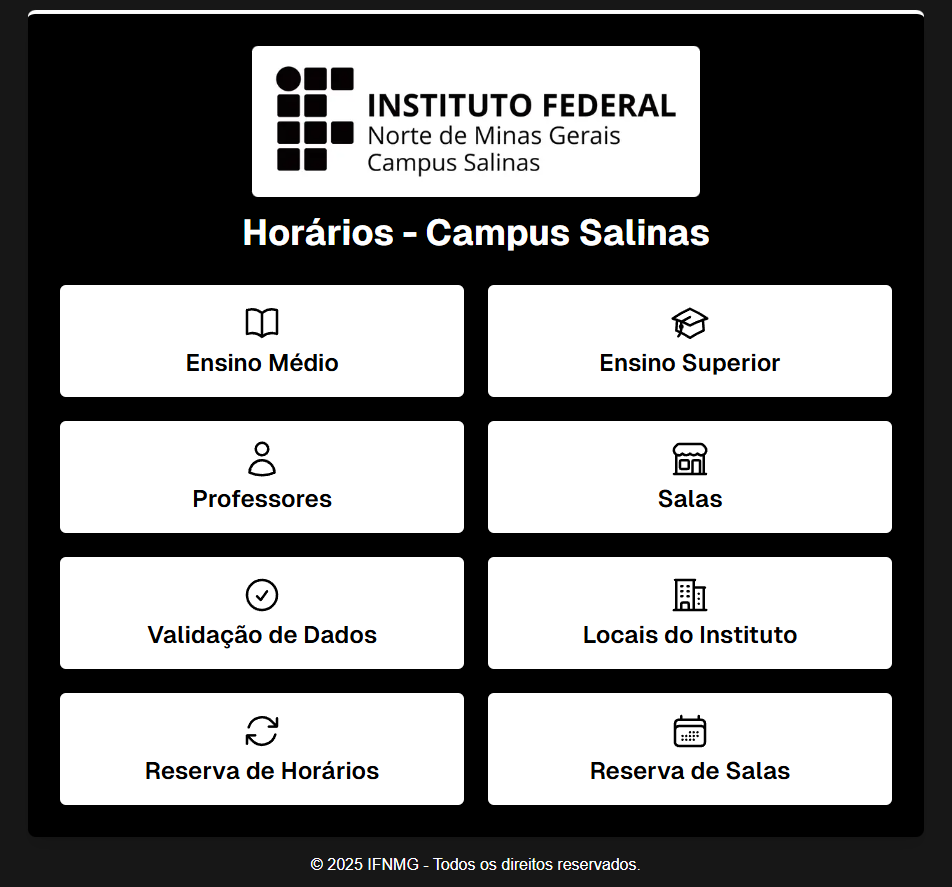
\includegraphics[width=1\textwidth]{Figuras/front-15.png}
        \caption*{Fonte: Elaborado pelo autor (2025)}
        \label{fig_front_15}
    \end{figure}

    \item \textbf{Responsividade}: garante que a interface funcione bem tanto em dispositivos móveis quanto em desktops, mantendo a usabilidade e a organização dos elementos. Apresentado na Figura \ref{fig_front_16}.

    \begin{figure}[H]
        \centering
        \caption{Responsividade}
        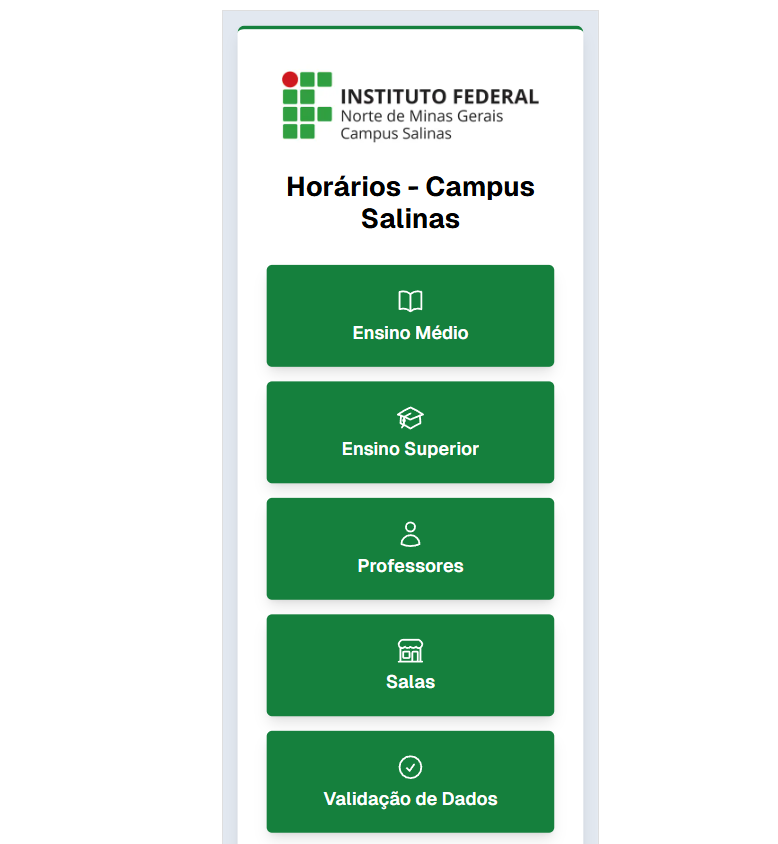
\includegraphics[width=0.7\textwidth]{Figuras/front-16.png}
        \caption*{Fonte: Elaborado pelo autor (2025)}
        \label{fig_front_16}
    \end{figure}
    
    \item \textbf{Busca de horários de cursos}: possibilita consultar os horários dos cursos técnicos e superiores, exibindo os cursos em uma lista suspensa. Apresentado na Figura \ref{fig_front_17}.

    \begin{figure}[htb]
        \centering
        \caption{Busca de horários dos cursos técnicos e superiores}
        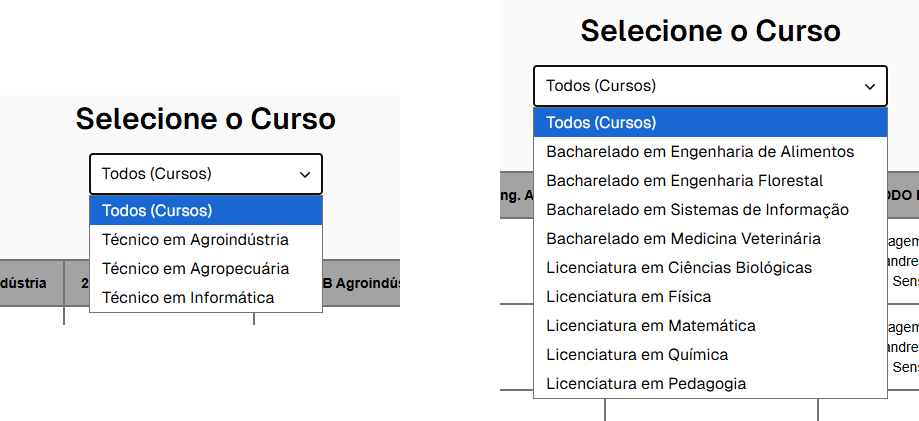
\includegraphics[width=0.7\textwidth]{Figuras/front-17.png}
        \caption*{Fonte: Elaborado pelo autor (2025)}
        \label{fig_front_17}
    \end{figure}
    
    \item \textbf{Busca de horários de professores}: permite selecionar um professor em uma lista suspensa e visualizar os horários. Apresentado na Figura \ref{fig_front_18}.

    \begin{figure}[htb]
        \centering
        \caption{Busca de horários de professores}
        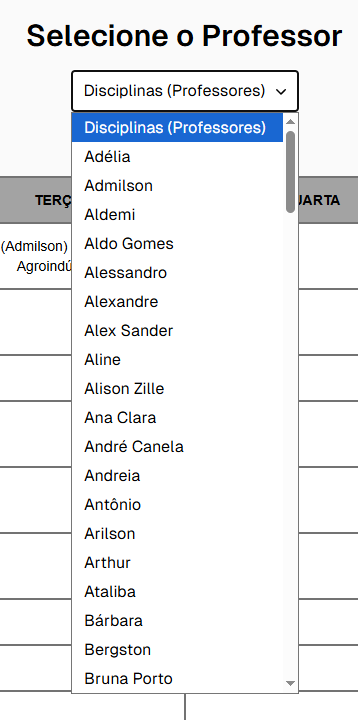
\includegraphics[width=0.6\textwidth]{Figuras/front-18.png}
        \caption*{Fonte: Elaborado pelo autor (2025)}
        \label{fig_front_18}
    \end{figure}
    
    \item \textbf{Busca de horários de salas}: permite selecionar uma sala em uma lista suspensa e visualizar os horários de ocupação. Apresentado na Figura \ref{fig_front_19}.

    \begin{figure}[htb]
        \centering
        \caption{Busca de horários de salas}
        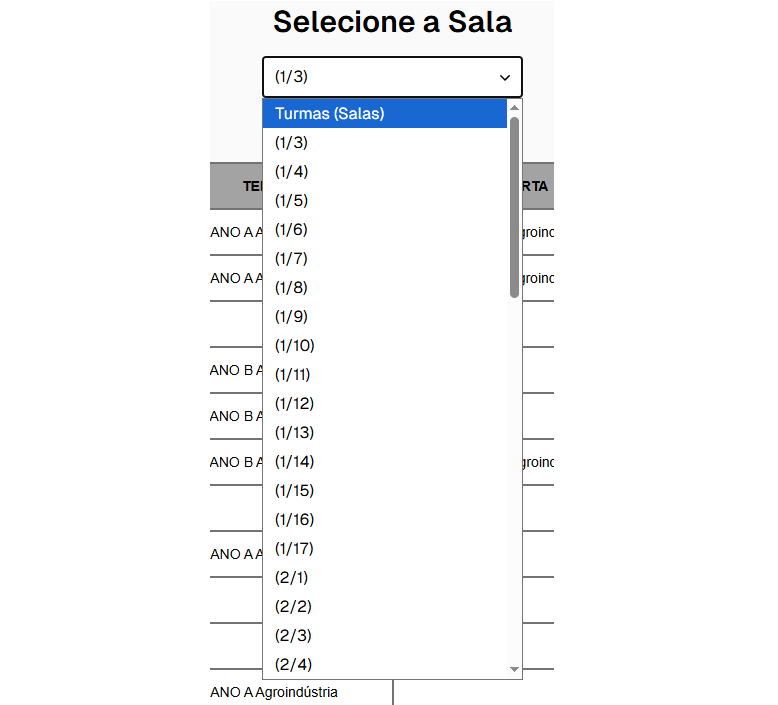
\includegraphics[width=0.5\textwidth]{Figuras/front-19.png}
        \caption*{Fonte: Elaborado pelo autor (2025)}
        \label{fig_front_19}
    \end{figure}
    
    \item \textbf{Download em PDF}: permite o usuário salvar a tabela dos horários em um arquivo no formato PDF, facilitando o acesso offline às informações. Apresentado na Figura \ref{fig_front_20}.

    \begin{figure}[htb]
        \centering
        \caption{Download em PDF}
        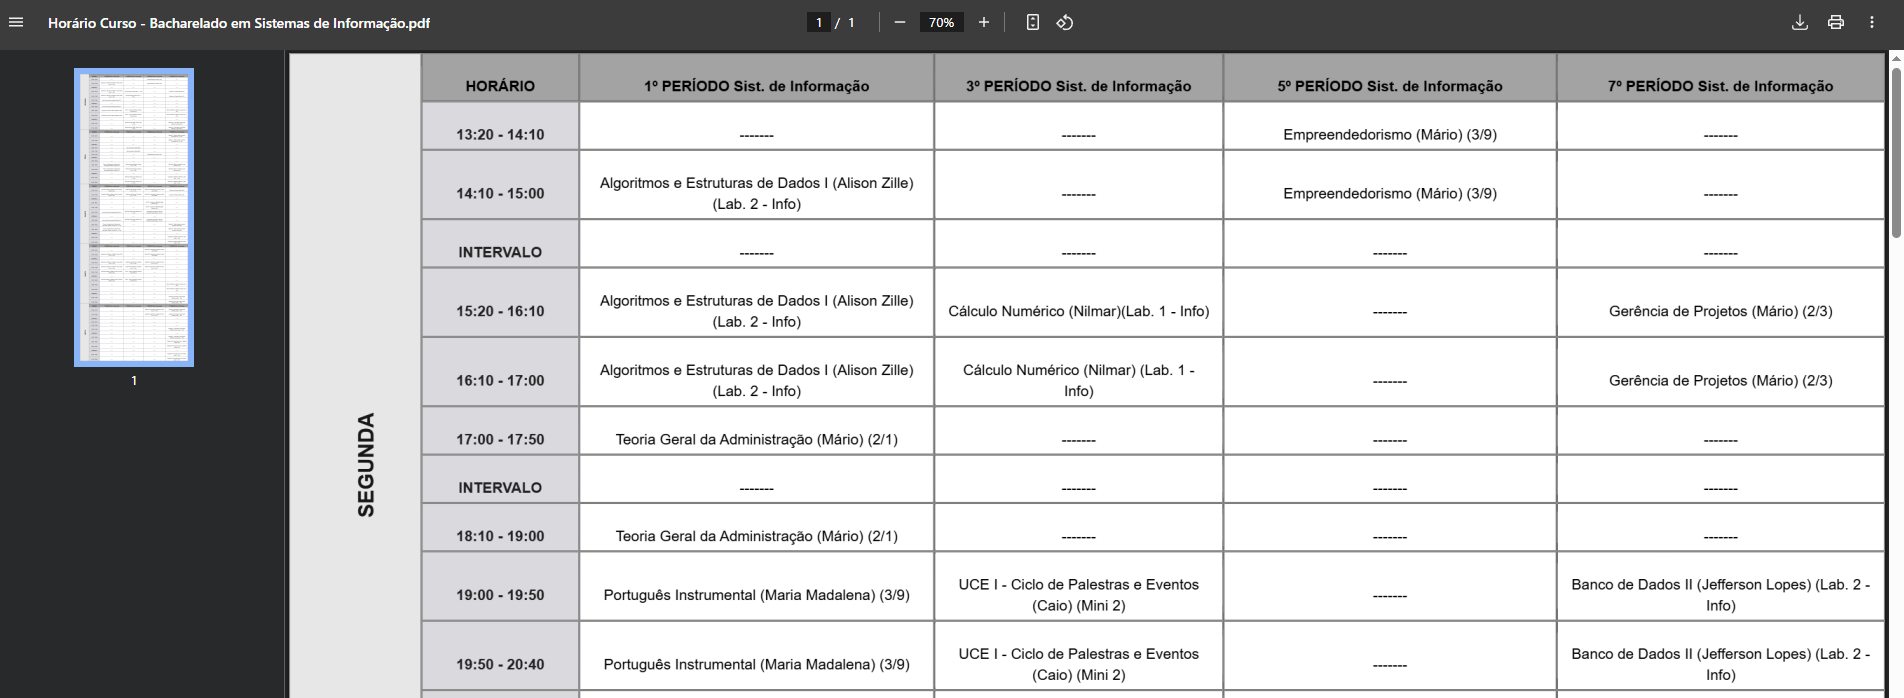
\includegraphics[width=0.9\textwidth]{Figuras/front-20.png}
        \caption*{Fonte: Elaborado pelo autor (2025)}
        \label{fig_front_20}
    \end{figure}
    
    \item \textbf{Tela de login}: restringe o acesso à tela de validação de dados apenas aos administradores, por meio de autenticação com usuário e senha. Apresentado na Figura \ref{fig_front_21}.

    \begin{figure}[htb]
        \centering
        \caption{Tela de login com credenciais incorretas}
        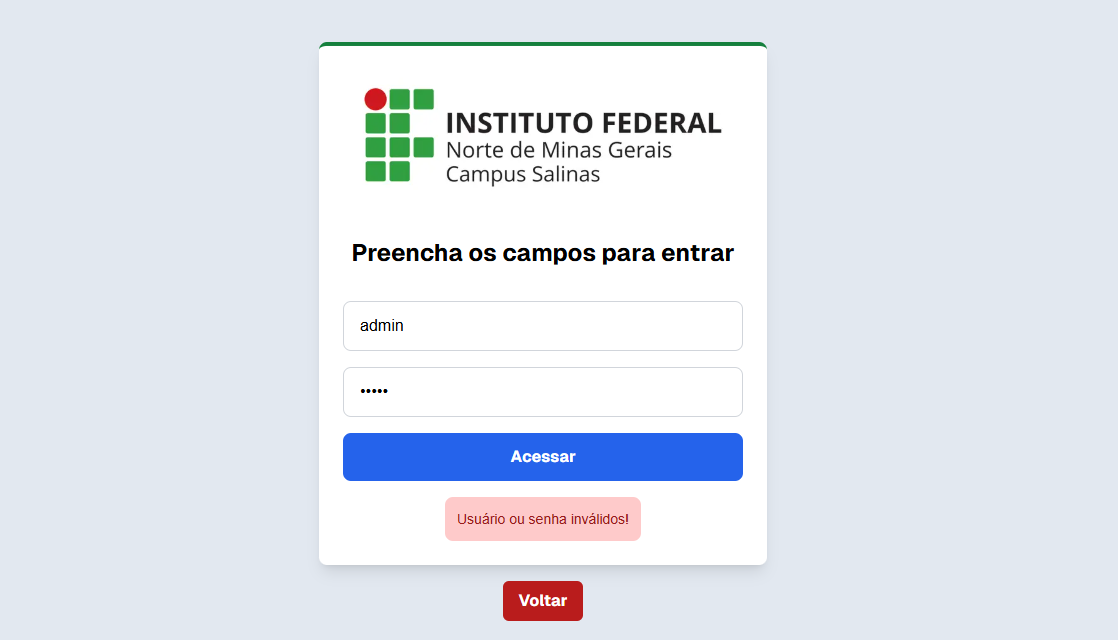
\includegraphics[width=0.8\textwidth]{Figuras/front-21.png}
        \caption*{Fonte: Elaborado pelo autor (2025)}
        \label{fig_front_21}
    \end{figure}
    
    \item \textbf{Tela de validação}: apresenta os resultados da verificação da planilha dos horários por meio de uma tabela com indicadores de conformidade, exibindo ``SIM'' ou ``NÃO'' para cada item validado. O processo de validação realiza as seguintes verificações:
    \begin{enumerate}
        \item Verificar a presença da guia \textit{Horário - Ensino Médio} que contém os horários das turmas dos cursos técnicos.
        \item Verificar a presença da guia \textit{Horário - Graduação} que contém os horários das turmas dos cursos superiores.
        \item Verificar a presença da guia \textit{Validação de Dados} que reúne a lista de professores da instituição.
        \item Validar se o intervalo de células B2:V76 está presente na guia \textit{Horário - Ensino Médio}.
        \item Validar se o intervalo de células B2:AW106 está presente na guia \textit{Horário - Graduação}.
        \item Validar se o intervalo de células A2:A está presente na guia \textit{Validação de Dados}.
        \item Avaliar a formatação das células, verificando se contêm os parênteses exigidos e se os nomes das turmas não apresentam parênteses. Se forem encontradas inconsistências, a tela exibe as células problemáticas, informando a guia, coluna e linha correspondentes.
    \end{enumerate}

    Ao final da página, é exibida uma mensagem com o resultado final da validação de dados. Caso todas as verificações sejam concluídas com êxito, a planilha é considerada em ótimo estado. Se forem identificados problemas, a mensagem informa que foram encontradas inconsistências que precisam ser corrigidas. Quando ocorre alguma falha durante o processo, a mensagem indica que houve um erro ao realizar a validação da planilha. Essa funcionalidade é apresentada nas Figuras \ref{fig_front_22}, \ref{fig_front_23} e \ref{fig_front_24}.

    \begin{figure}[htb]
        \centering 
        \caption{Tela de validação com resultado de sucesso}
        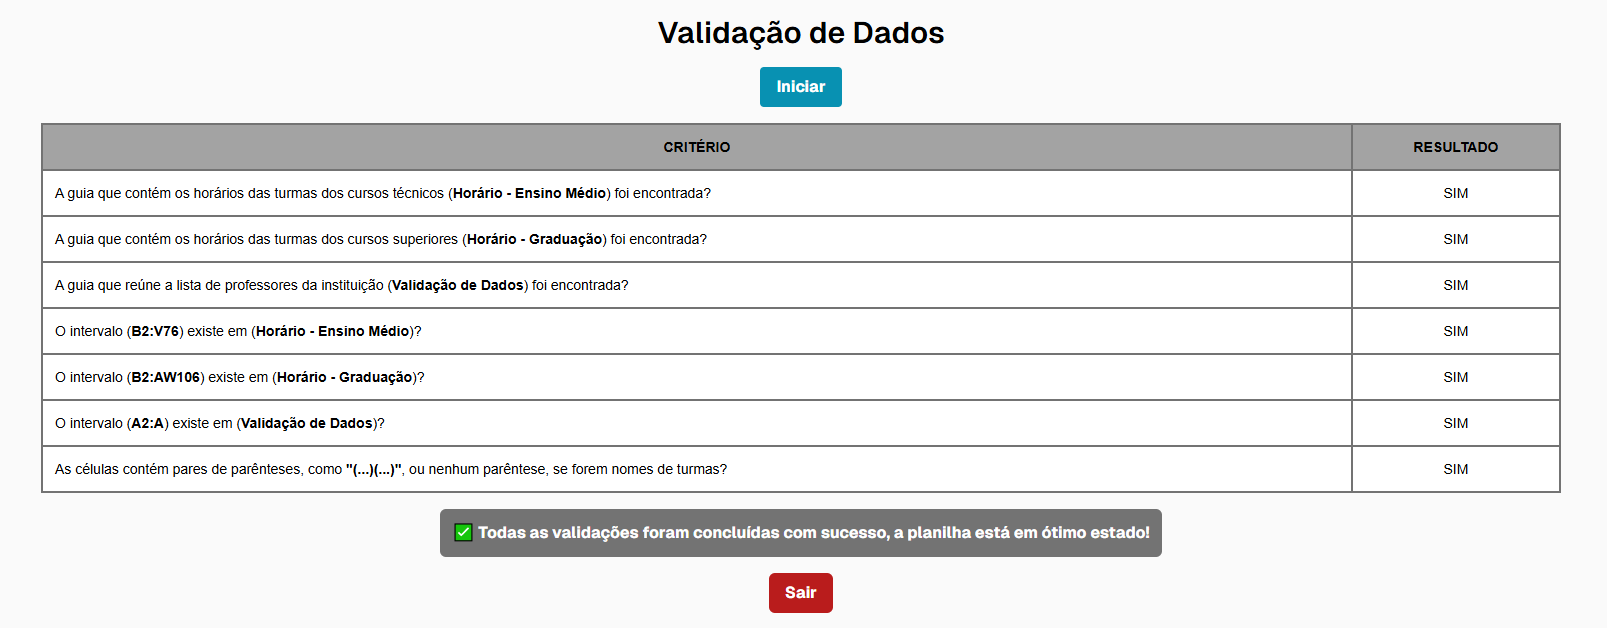
\includegraphics[width=1\textwidth]{Figuras/front-22.png}
        \caption*{Fonte: Elaborado pelo autor (2025)}
        \label{fig_front_22}
    \end{figure}

    \begin{figure}[H]
        \centering
        \caption{Tela de validação com resultado mostrando inconsistências}
        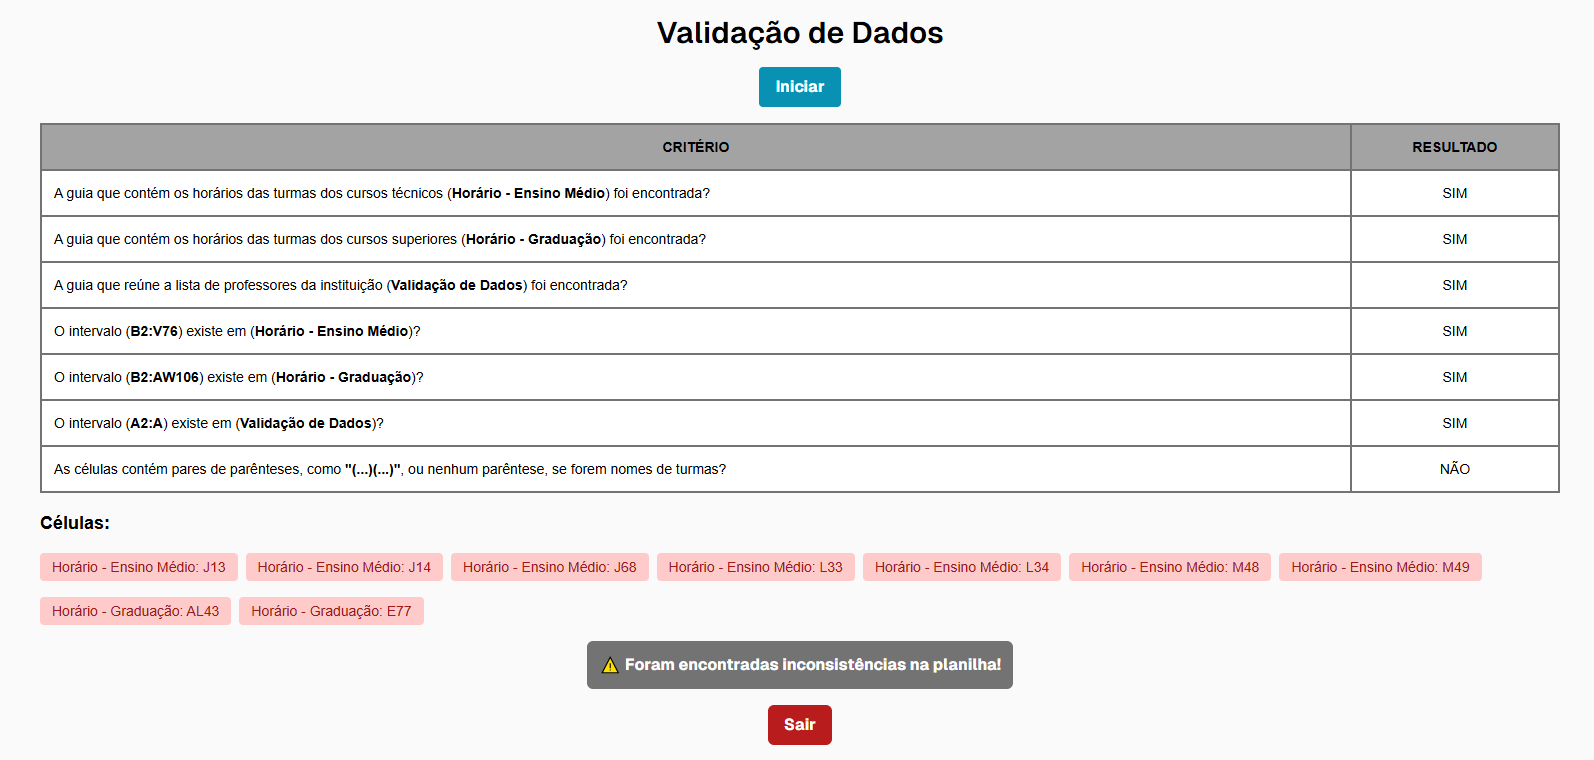
\includegraphics[width=1\textwidth]{Figuras/front-23.png}
        \caption*{Fonte: Elaborado pelo autor (2025)}
        \label{fig_front_23}
    \end{figure}

    \begin{figure}[htb]
        \centering
        \caption{Tela de validação com resultado de erro}
        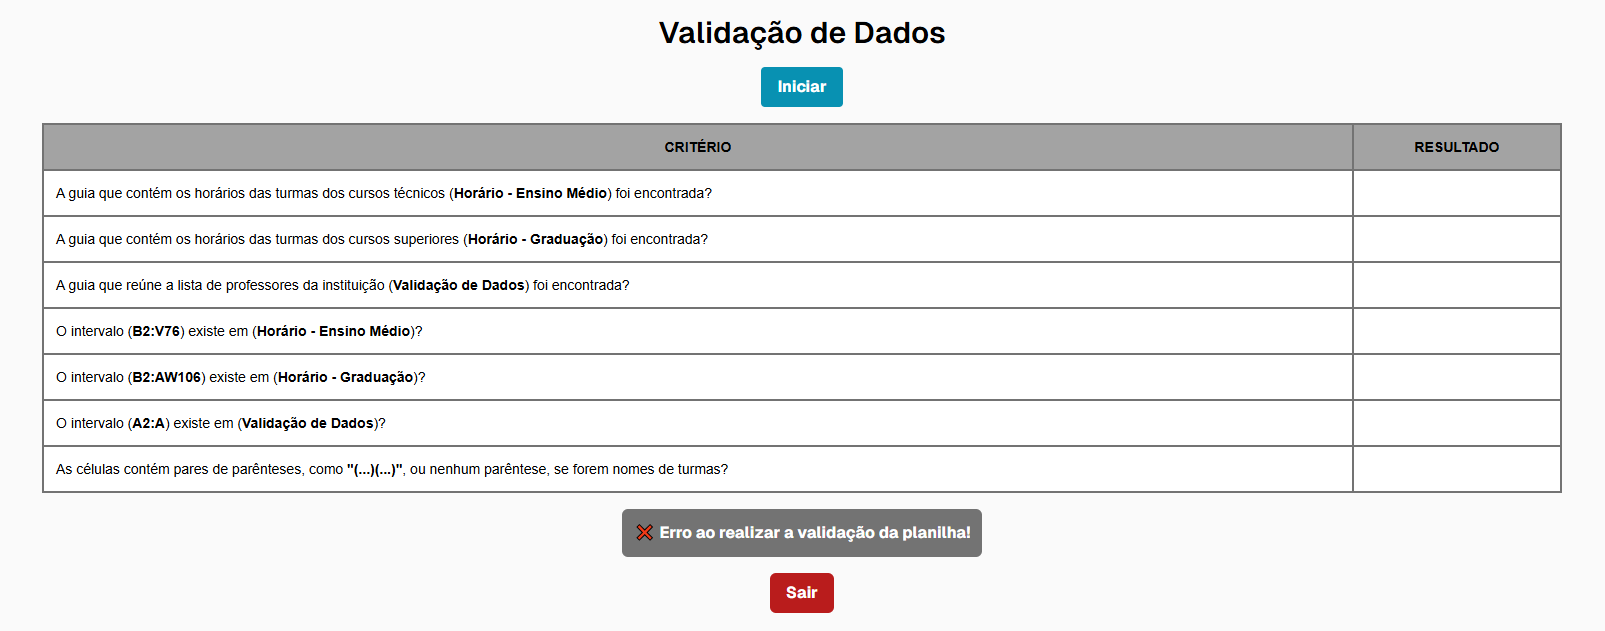
\includegraphics[width=1\textwidth]{Figuras/front-24.png}
        \caption*{Fonte: Elaborado pelo autor (2025)}
        \label{fig_front_24}
    \end{figure}
\end{itemize}

\section{Back-end}

\subsection{Google Sheets como Banco de Dados}

O sistema utiliza duas planilhas hospedadas no \textit{Google Sheets}. A primeira planilha contém duas guias com os horários acadêmicos e a uma guia com a lista dos professores disponíveis, conforme apresentado a seguir:

\begin{figure}[H]
    \centering
    \caption{Guia ``Horário - Ensino Médio''}
    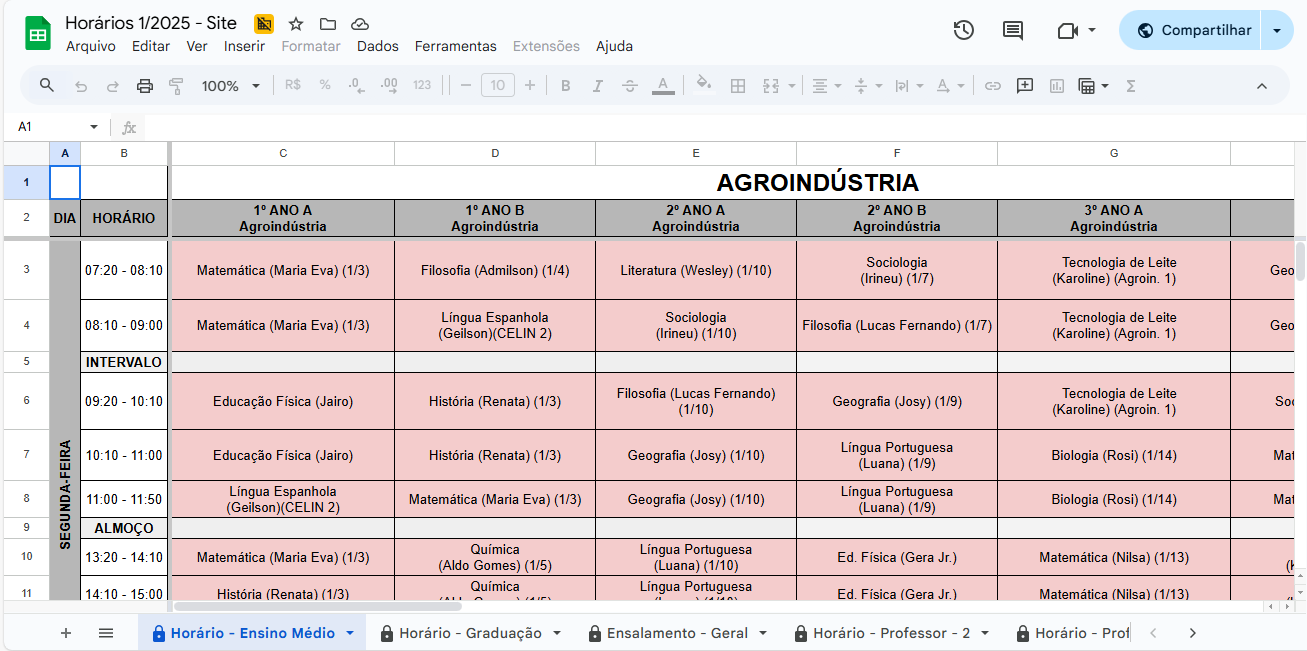
\includegraphics[width=0.9\textwidth]{Figuras/plan-1.png}
    \caption*{Fonte: Elaborado pelo autor (2025)}
    \label{fig_plan_1}
\end{figure}

A Figura \ref{fig_plan_1} mostra a guia que contém os horários das turmas dos cursos técnicos, distribuídos no intervalo de células B2:V76.

\begin{figure}[htb]
    \centering
    \caption{Guia ``Horário - Graduação''}
    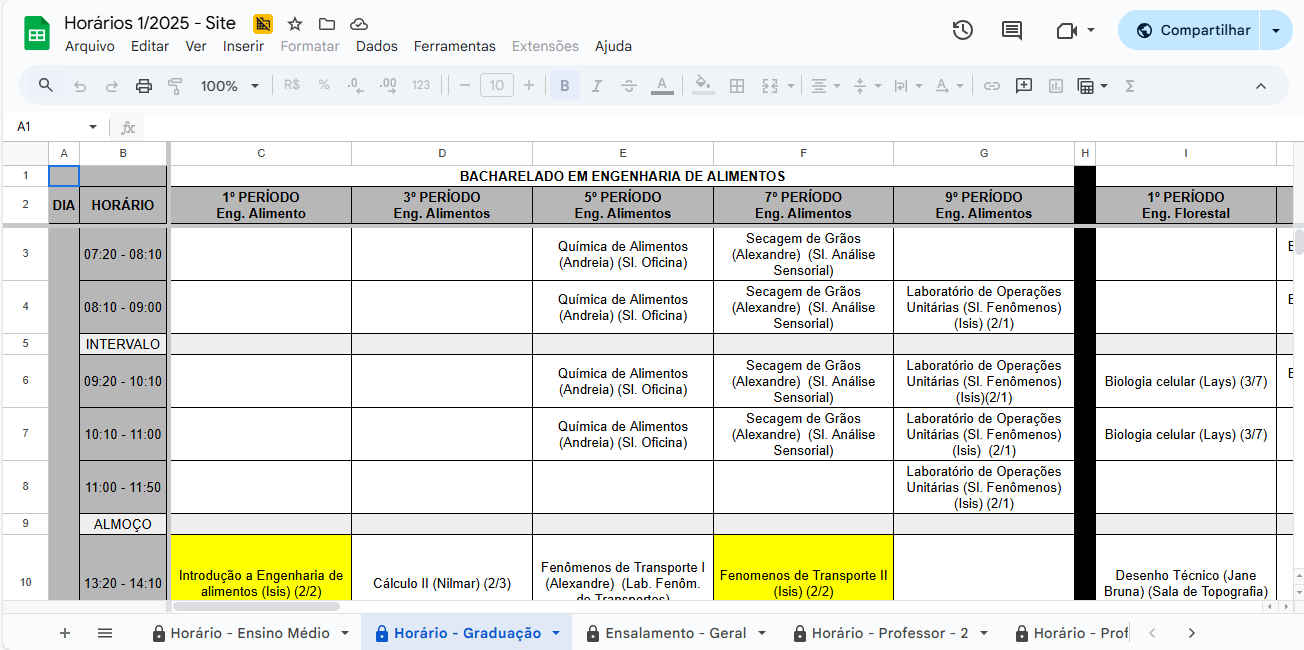
\includegraphics[width=0.9\textwidth]{Figuras/plan-2.png}
    \caption*{Fonte: Elaborado pelo autor (2025)}
    \label{fig_plan_2}
\end{figure}

A Figura \ref{fig_plan_2} mostra a guia que contém os horários das turmas dos cursos superiores, distribuídos no intervalo de células B2:AW106.

\begin{figure}[H]
    \centering
    \caption{Guia ``Validação de Dados''}
    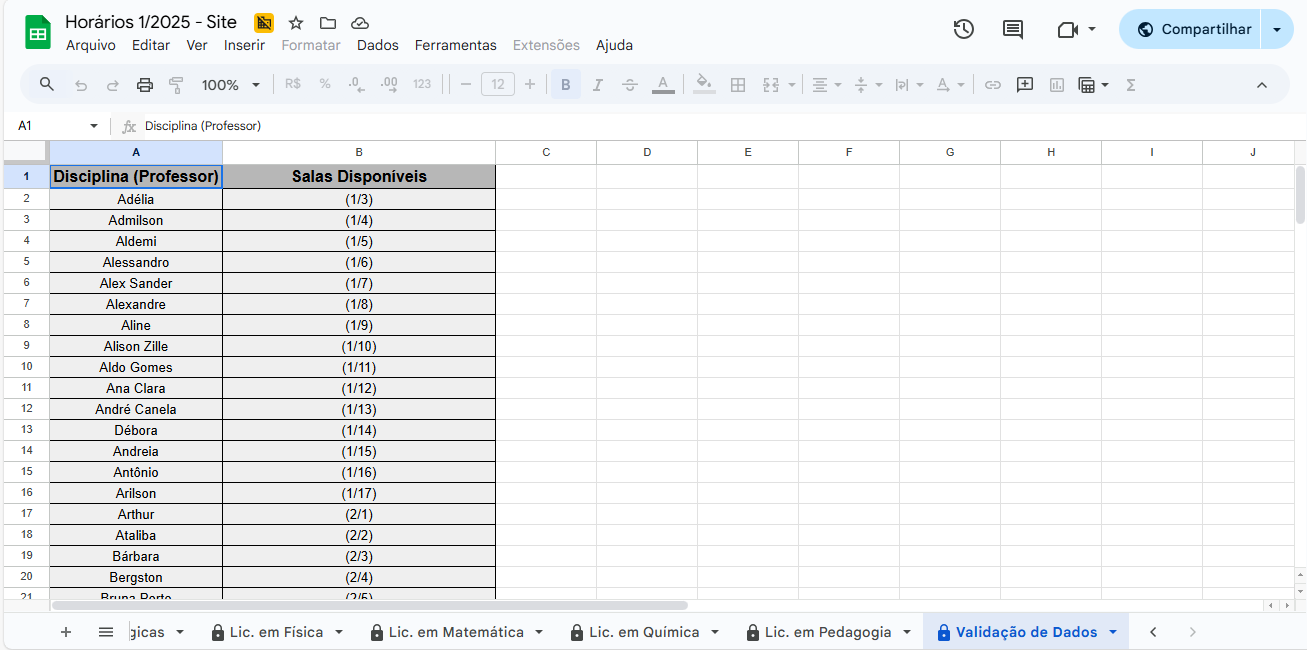
\includegraphics[width=0.9\textwidth]{Figuras/plan-3.png}
    \caption*{Fonte: Elaborado pelo autor (2025)}
    \label{fig_plan_3}
\end{figure}

A Figura \ref{fig_plan_3}, mostra a guia que reúne a lista de professores da instituição, distribuídos no intervalo de células A2:A.

A segunda planilha contém uma guia com as credenciais de login necessárias para autenticação:

\begin{figure}[htb]
    \centering
    \caption{Guia ``Login''}
    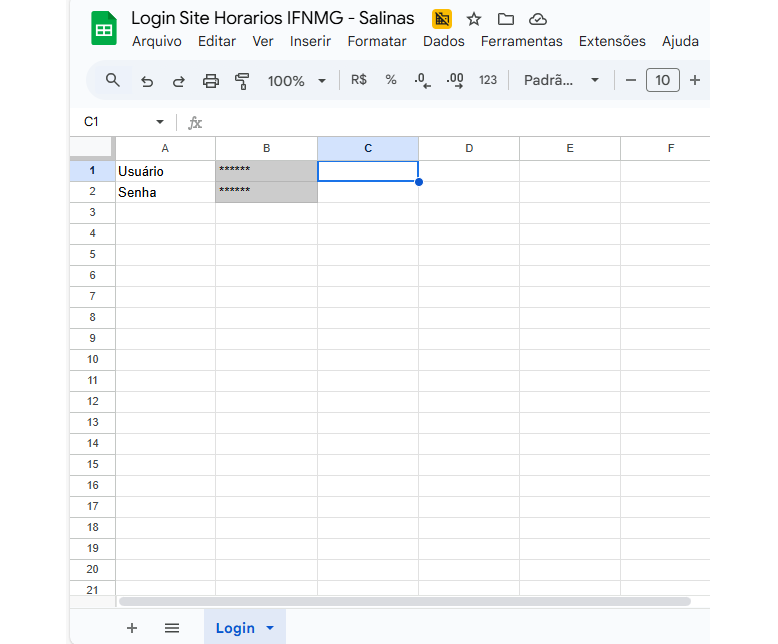
\includegraphics[width=0.75\textwidth]{Figuras/plan-4.png}
    \caption*{Fonte: Elaborado pelo autor (2025)}
    \label{fig_plan_4}
\end{figure}

A Figura \ref{fig_plan_4} mostra a guia da planilha com as credenciais de login para acessar a tela de validação de dados, contendo os campos de usuário e senha, distribuídos no intervalo de células B1:B2.

\subsection{Desenvolvimento do Back-end}

O \textit{back-end} foi desenvolvido com a linguagem \textit{Java} e o \textit{Spring Framework}. Essa tecnologia possibilitou integrar de forma segura a \textit{API} do \textit{Google Sheets}, garantindo a leitura dos dados necessários para o funcionamento da plataforma e enviando essas informações ao \textit{front-end} de maneira estruturada e confiável. Todo o processo priorizou simplicidade na configuração e facilidade de manutenção, permitindo atender às demandas do projeto com eficiência. O código está disponível no repositório do projeto em: \url{https://github.com/ifnmgsal-inf/Horarios-IFNMG-Salinas/tree/main/backend}.

\subsection{Estrutura do Back-end}

A estrutura do \textit{back-end} está organizada seguindo o padrão arquitetural MVC, o que favorece a separação de responsabilidades, facilita a manutenção e a evolução do sistema. Na Figura \ref{fig_back_1}, destacam-se os principais elementos do projeto:

\begin{figure}[htb]
    \centering
    \caption{Estrutura do back-end}
    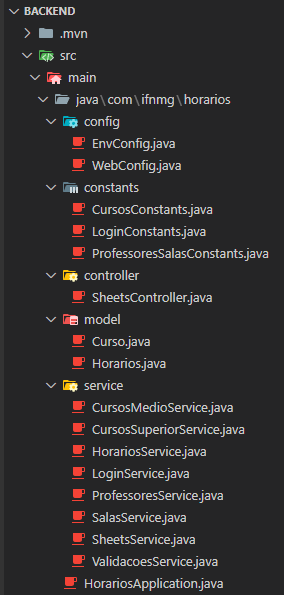
\includegraphics[width=0.9\textwidth]{Figuras/back-1.png}
    \caption*{Fonte: Elaborado pelo autor (2025)}
    \label{fig_back_1}
\end{figure}

\begin{itemize}
    \item \textbf{config}: pacote para armazenar classes de configuração do sistema, como a \textit{EnvConfig.java}, que define as variáveis de ambiente, e a \textit{WebConfig.java}, responsável por ajustes na configuração do \textit{Spring Boot}, incluindo a definição do CORS. Um mecanismo que define quais origens externas podem se comunicar com a \textit{API}, permitindo uma integração segura entre o \textit{front-end} e o \textit{back-end}, mesmo em domínios diferentes.
    \item \textbf{constants}: pacote para centralizar valores fixos e listas, contendo as classes \textit{CursosConstants.java}, \textit{LoginConstants.java} e \textit{ProfessoresSalasConstants.java}, que mantêm os dados de cursos, professores, salas e credenciais de login.
    \item \textbf{controller}: pacote para controlar as requisições recebidas e encaminhá-las para os serviços adequados, abrigando a classe \textit{SheetsController.java}, que gerencia as rotas da aplicação.
    \item \textbf{model}: pacote para definir as classes de domínio que representam a estrutura dos dados, como \textit{Curso.java} e \textit{Horarios.java}, que servem de modelo para a manipulação das informações obtidas do \textit{Google Sheets}.
    \item \textbf{service}: pacote para concentrar as regras de negócio e a comunicação com a \textit{API} do \textit{Google Sheets}, incluindo as classes \textit{CursosMedioService.java}, \textit{CursosSuperiorService.java}, \textit{HorariosService.java}, \textit{LoginService.java}, \textit{ProfessoresService.java}, \textit{SalasService.java}, \textit{SheetsService.java} e \textit{ValidacoesService.java}.
    \item \textbf{HorariosApplication.java}: classe principal que executa a aplicação \textit{Spring Boot} e carrega as configurações do sistema.
\end{itemize}

\subsection{Funcionalidades do Back-end}

\begin{itemize}
    \item \textbf{Estabelecer a conexão com a API do Google Sheets}: para coletar os dados das planilhas utilizadas como banco de dados. Essa função é executada pela classe \textit{SheetsService.java}, que gerencia a integração entre o \textit{back-end} e o serviço do Google, possibilitando o acesso dinâmico e estruturado às informações necessárias para o funcionamento da plataforma.
    
    \begin{figure}[H]
        \centering
        \caption{Classe ``SheetsService.java''}
        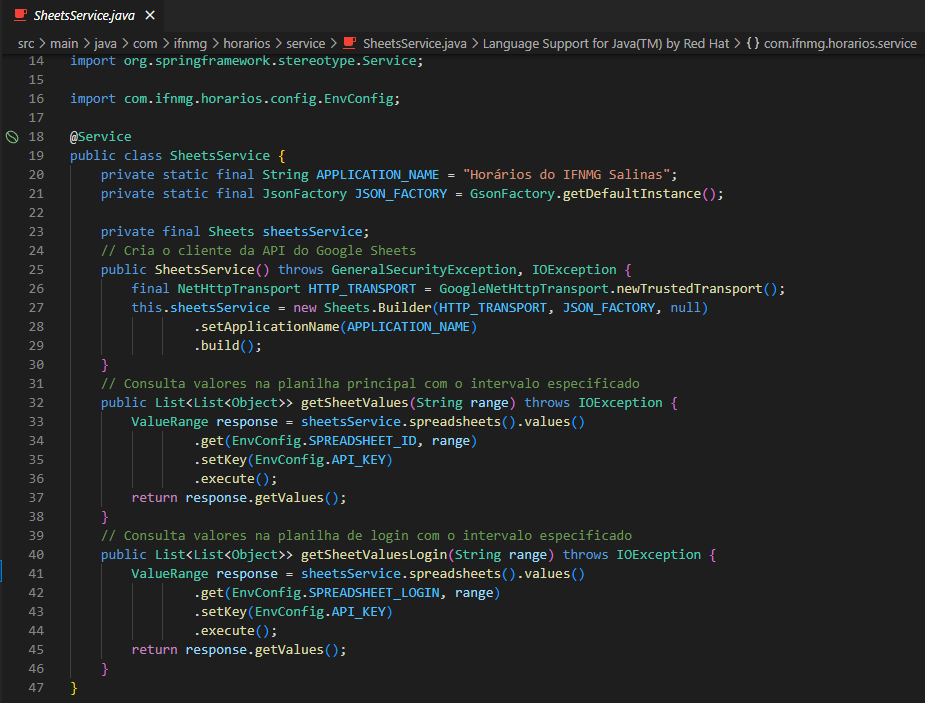
\includegraphics[width=1\textwidth]{Figuras/back-2.png}
        \caption*{Fonte: Elaborado pelo autor (2025)}
        \label{fig_back_2}
    \end{figure}
    
    A Figura \ref{fig_back_2} mostra a classe \textit{SheetsService.java}. A seguir, estão descritas suas principais funcionalidades:

    \begin{itemize}
        \item \textbf{Constantes}: \textit{APPLICATION\_NAME} e \textit{JSON\_FACTORY} são utilizadas para configurar a instância da \textit{API} do \textit{Google Sheets}. O nome da aplicação é definido para identificação no console da \textit{API}, e o \textit{JsonFactory} especifica o formato de serialização dos dados trafegados entre o \textit{back-end} e o serviço do Google.
        \item \textbf{Construtor SheetsService()}: Responsável por configurar a instância do cliente da \textit{API} do \textit{Google Sheets}, que é armazenada no atributo sheetsService. Para isso, é utilizada uma conexão segura, criada com \textit{GoogleNetHttpTransport}, garantindo uma comunicação autenticada e confiável entre o sistema e a \textit{API}.
        \item \textbf{Método getSheetValues(String range)}: Realiza a leitura dos dados da planilha principal, onde estão os horários acadêmicos, com base no intervalo informado pelo parâmetro \textit{range}. O método utiliza duas variáveis de ambiente:
        \begin{itemize}
            \item \textbf{EnvConfig.SPREADSHEET\_ID}: \textit{ID} da planilha com os horários acadêmicos.
            \item \textbf{EnvConfig.API\_KEY}: chave de \textit{API} do \textit{Google Sheets}.
        \end{itemize}
        \item \textbf{Método getSheetValuesLogin(String range)}: Realiza a leitura dos dados da planilha de login, com base no intervalo informado pelo parâmetro \textit{range}. Esse método é executado antes do acesso à tela de validação de dados, sendo responsável por autenticar o usuário na tela de login. As variáveis de ambiente utilizadas são:
        \begin{itemize}
            \item \textbf{EnvConfig.SPREADSHEET\_LOGIN}: \textit{ID} da planilha com as credenciais de login.
            \item \textbf{EnvConfig.API\_KEY}: mesma chave de \textit{API} do \textit{Google Sheets} em uso no método anterior.
        \end{itemize}
    \end{itemize}

    \item \textbf{Disponibilizar endpoints REST}: para consultar horários acadêmicos e resultados de validação de dados, assegurando respostas padronizadas e consistentes. Essa funcionalidade é implementada na classe \textit{SheetsController}, que organiza e define as rotas de acesso dos dados. As rotas são definidas exclusivamente com o método GET, uma vez que o sistema realiza apenas operações de leitura, sem modificar os dados. Cada rota é mapeada para um método específico do \textit{controller}, responsável por retornar as informações de forma estruturada por meio do objeto \textit{ResponseEntity}. A seguir, são descritos os principais \textit{endpoints} da aplicação.

    \begin{figure}[htb]
        \centering
        \caption{Endpoint de consulta dos horários dos cursos técnicos}
        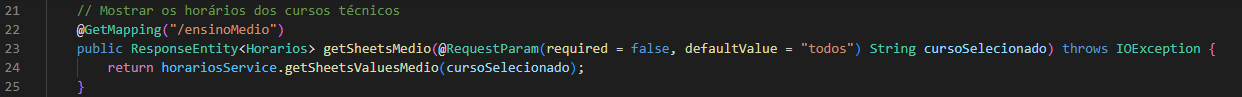
\includegraphics[width=0.9\textwidth]{Figuras/back-3.png}
        \caption*{Fonte: Elaborado pelo autor (2025)}
        \label{fig_back_3}
    \end{figure}

    O objetivo do \textit{endpoint} apresentado na Figura \ref{fig_back_3} é retornar os horários dos cursos técnicos. O parâmetro utilizado é \textit{cursoSelecionado}, que é opcional e por padrão assume o valor \textit{todos}. Tendo isso como referência, o sistema consulta os dados na planilha e os retorna de forma organizada dentro de um objeto \textit{Horarios} com os horários de todos os cursos técnicos ou de um curso técnico específico.

    \begin{figure}[htb]
        \centering
        \caption{Endpoint de consulta dos horários dos cursos superiores}
        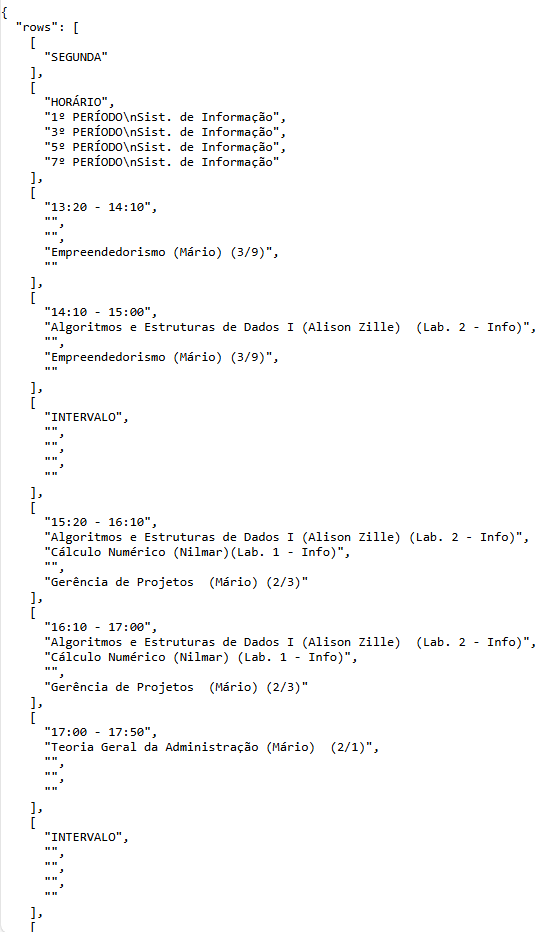
\includegraphics[width=0.9\textwidth]{Figuras/back-4.png}
        \caption*{Fonte: Elaborado pelo autor (2025)}
        \label{fig_back_4}
    \end{figure}

    O objetivo do \textit{endpoint} apresentado na Figura \ref{fig_back_4} é retornar os horários dos cursos superiores. O parâmetro utilizado é \textit{cursoSelecionado}, que é opcional e por padrão assume o valor \textit{todos}. Tendo isso como referência, o sistema consulta os dados na planilha e os retorna de forma organizada dentro de um objeto \textit{Horarios} com os horários de todos os cursos superiores ou de um curso superior específico.

    \begin{figure}[htb]
        \centering
        \caption{Endpoint de consulta dos horários dos professores}
        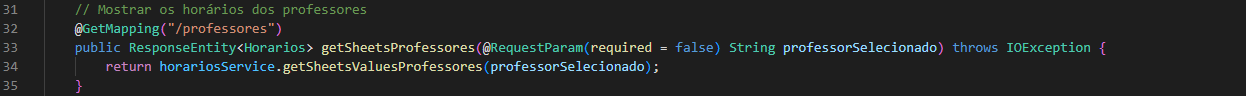
\includegraphics[width=0.9\textwidth]{Figuras/back-5.png}
        \caption*{Fonte: Elaborado pelo autor (2025)}
        \label{fig_back_5}
    \end{figure}

    Conforme ilustrado na Figura \ref{fig_back_5}, o objetivo do \textit{endpoint} é retornar os horários dos professores. O parâmetro \textit{professorSelecionado} é opcional e pode ser deixado em branco. Com base nisso, o sistema consulta os dados na planilha e os retorna de forma organizada dentro de um objeto \textit{Horarios} com os horários de um professor específico.

    \begin{figure}[htb]
        \centering
        \caption{Endpoint de consulta dos horários de ocupação das salas}
        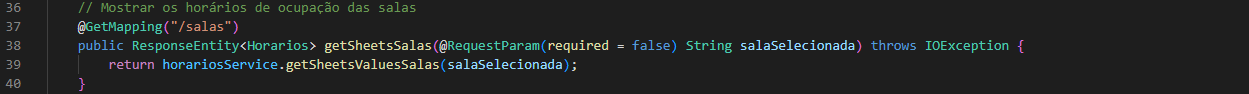
\includegraphics[width=0.9\textwidth]{Figuras/back-6.png}
        \caption*{Fonte: Elaborado pelo autor (2025)}
        \label{fig_back_6}
    \end{figure}

    Conforme ilustrado na Figura \ref{fig_back_6}, o objetivo do \textit{endpoint} é retornar os horários de ocupação das salas. O parâmetro \textit{salaSelecionada} é opcional e pode ser deixado em branco. Com base nisso, o sistema consulta os dados na planilha e os retorna de forma organizada dentro de um objeto \textit{Horarios} com os horários de ocupação de uma sala específica.

    \begin{figure}[H]
        \centering
        \caption{Endpoint de consulta das permissões para visualizar validação da planilha}
        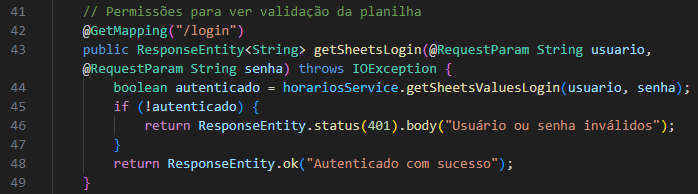
\includegraphics[width=0.9\textwidth]{Figuras/back-7.png}
        \caption*{Fonte: Elaborado pelo autor (2025)}
        \label{fig_back_7}
    \end{figure}

    Como mostrado na Figura \ref{fig_back_7}, o objetivo do \textit{endpoint} é validar as credenciais de acesso informadas. Os parâmetros obrigatórios são \textit{usuario} e \textit{senha}. Com essas informações, o sistema realiza a autenticação e retorna uma mensagem com o código de estado HTTP correspondente, sendo 200 (\textit{OK}) em caso de sucesso ou 401 (\textit{Unauthorized}) quando as credenciais estão incorretas.

    \begin{figure}[htb]
        \centering
        \caption{Endpoint de consulta para validar dados da planilha}
        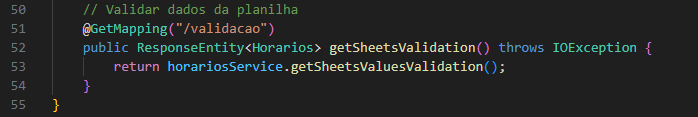
\includegraphics[width=0.9\textwidth]{Figuras/back-8.png}
        \caption*{Fonte: Elaborado pelo autor (2025)}
        \label{fig_back_8}
    \end{figure}

    Conforme mostrado na Figura \ref{fig_back_8}, o objetivo do \textit{endpoint} é retornar os resultados da validação dos dados da planilha de horários. Nenhum parâmetro é necessário para a execução da requisição. Ao ser acionado, o sistema analisa a planilha e responde com um objeto \textit{Horarios} contendo eventuais inconsistências ou erros detectados durante o processo de validação.
\end{itemize}

\section{Deploy}

A plataforma pode acessada no seguinte endereço: \url{https://horarios-ifnmg-salinas.vercel.app}. O \textit{front-end} foi hospedado na plataforma \textit{Vercel}, permitindo a disponibilização da interface do usuário com alta performance e integração contínua, como apresentado na Figura \ref{fig_deploy_1}.

\begin{figure}[H]
    \centering
    \caption{Deploy do front-end da plataforma na Vercel}
    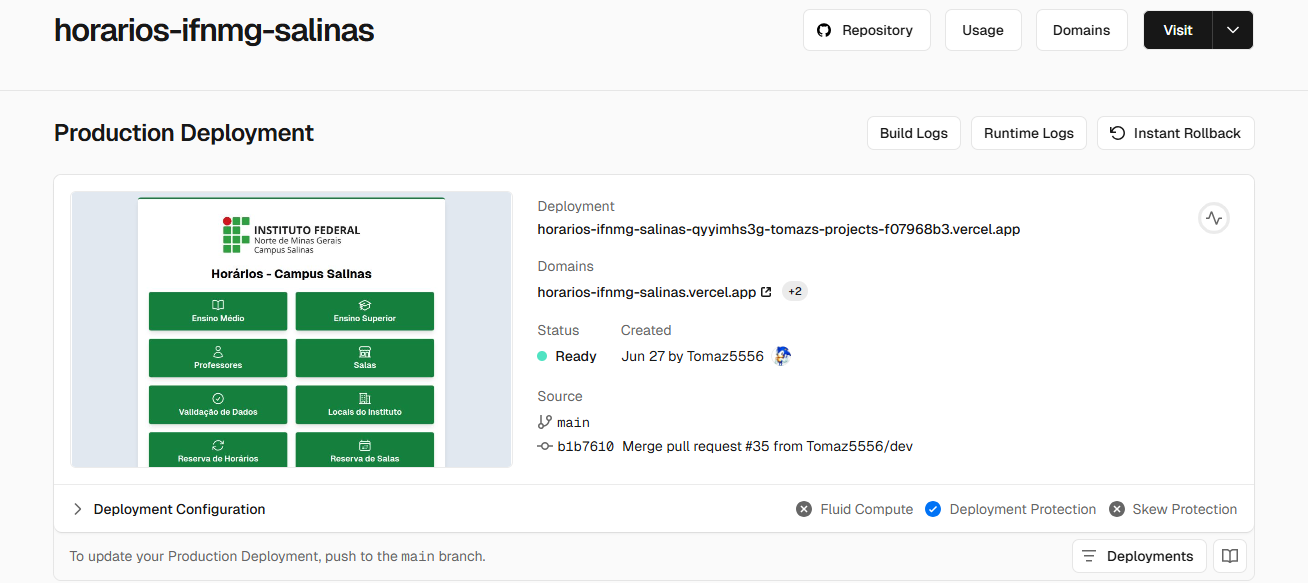
\includegraphics[width=1\textwidth]{Figuras/deploy-1.png}
    \caption*{Fonte: Elaborado pelo autor (2025)}
    \label{fig_deploy_1}
\end{figure}

Já o \textit{back-end} foi hospedado na plataforma \textit{Koyeb}, responsável por executar a \textit{API} que processa e envia os dados do \textit{Google Sheets} ao \textit{front-end}, conforme apresentado na Figura \ref{fig_deploy_2}.

\begin{figure}[htb]
    \centering
    \caption{Deploy do back-end da plataforma na Koyeb}
    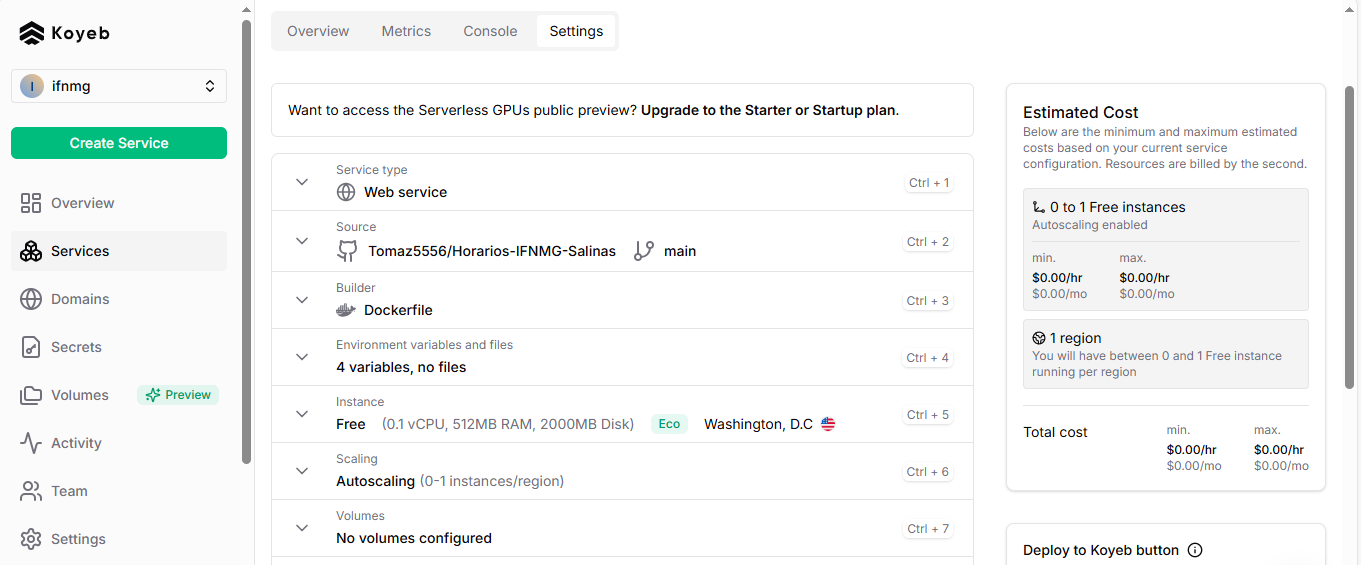
\includegraphics[width=1\textwidth]{Figuras/deploy-2.png}
    \caption*{Fonte: Elaborado pelo autor (2025)}
    \label{fig_deploy_2}
\end{figure}

\section{Documentação}

As Figuras \ref{fig_doc_1}, \ref{fig_doc_2}, \ref{fig_doc_3} e \ref{fig_doc_4} apresentam a documentação técnica elaborada para a planilha utilizada como banco de dados do sistema. A documentação está disponível no seguinte endereço: \url{https://ifnmgsal-inf.github.io/Horarios-IFNMG-Salinas}. Esse material descreve, de forma clara e objetiva, as instruções para atualização do identificador da planilha, as regras de preenchimento dos dados, bem como os padrões de nomes e intervalos de células necessários para garantir a integridade do funcionamento da plataforma.

\begin{figure}[htb]
    \centering
    \caption{Instruções para desenvolvedores}
    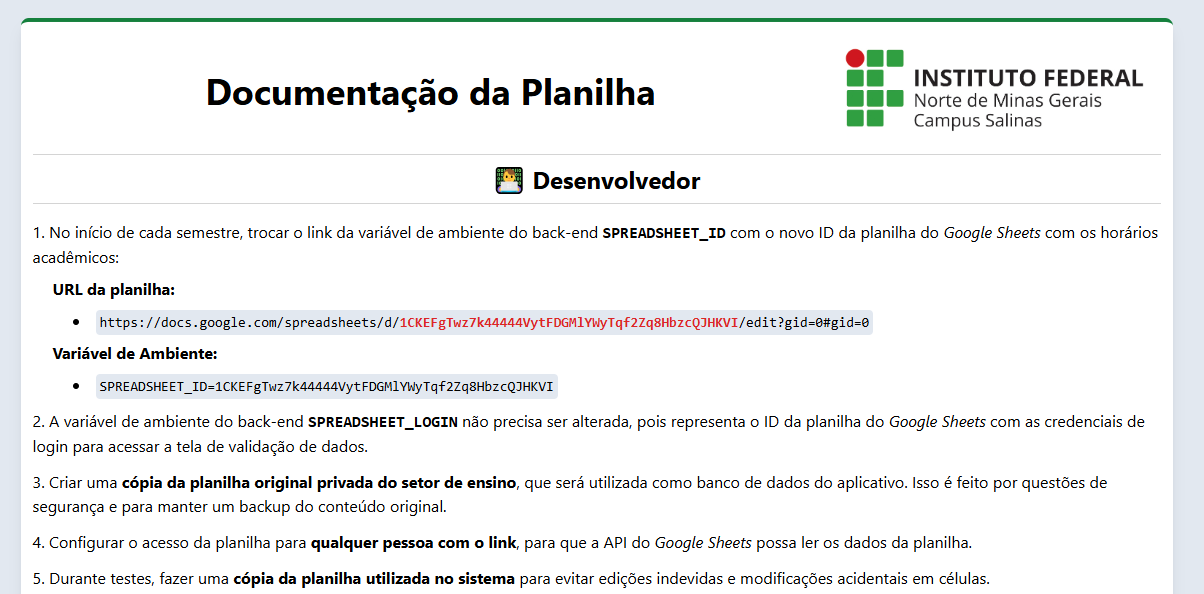
\includegraphics[width=0.9\textwidth]{Figuras/doc-1.png}
    \caption*{Fonte: Elaborado pelo autor (2025)}
    \label{fig_doc_1}
\end{figure}

\begin{figure}[htb]
    \centering
    \caption{Instruções para administradores da planilha}
    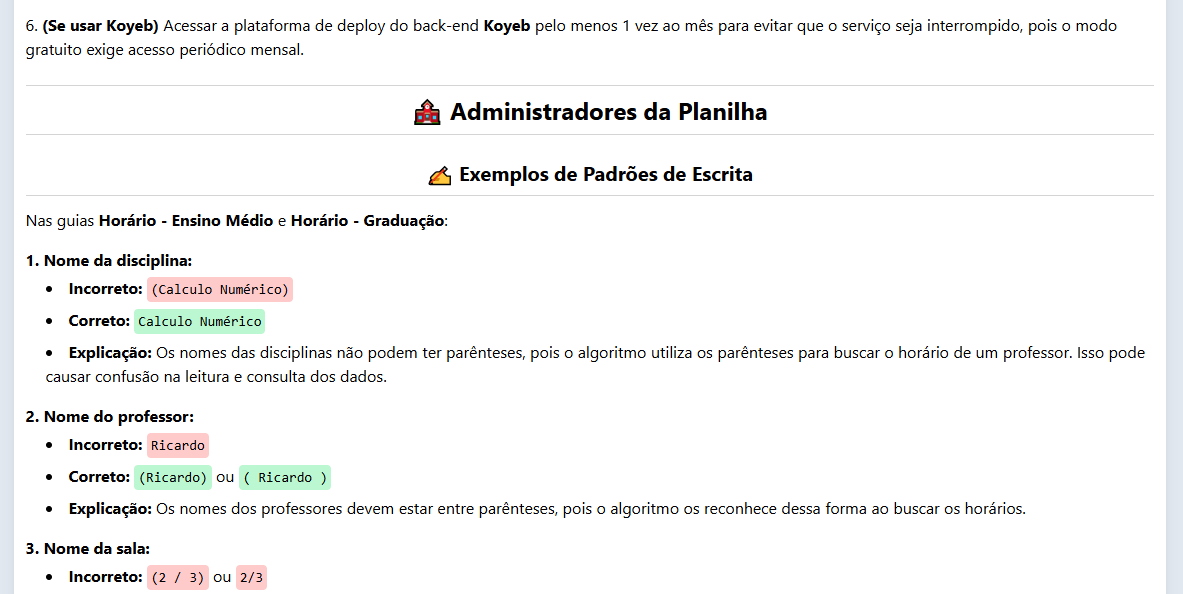
\includegraphics[width=0.9\textwidth]{Figuras/doc-2.png}
    \caption*{Fonte: Elaborado pelo autor (2025)}
    \label{fig_doc_2}
\end{figure}

\begin{figure}[htb]
    \centering
    \caption{Explicação das guias e intervalos de células}
    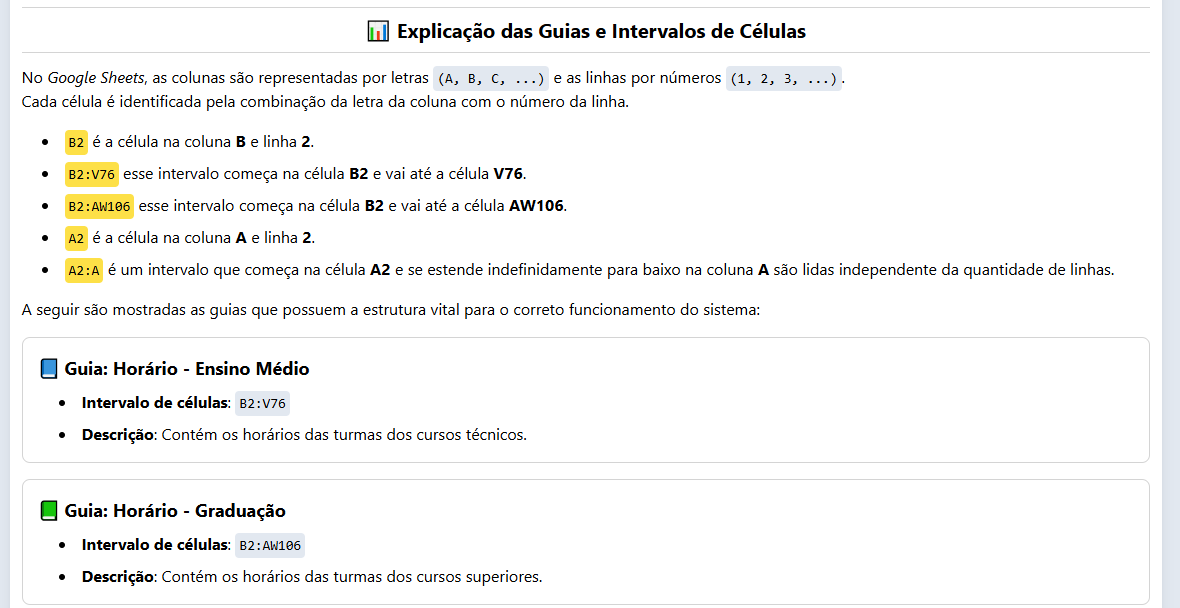
\includegraphics[width=0.9\textwidth]{Figuras/doc-3.png}
    \caption*{Fonte: Elaborado pelo autor (2025)}
    \label{fig_doc_3}
\end{figure}

\begin{figure}[htb]
    \centering
    \caption{Observação sobre mudanças estruturais}
    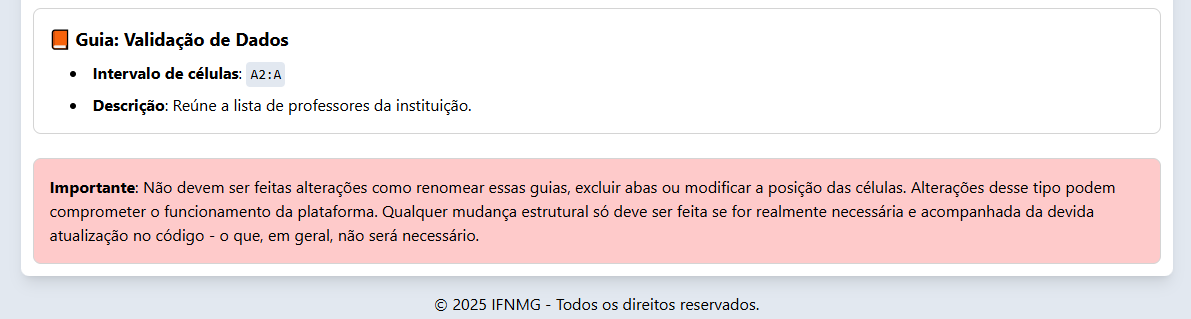
\includegraphics[width=0.9\textwidth]{Figuras/doc-4.png}
    \caption*{Fonte: Elaborado pelo autor (2025)}
    \label{fig_doc_4}
\end{figure}